% Options for packages loaded elsewhere
\PassOptionsToPackage{unicode}{hyperref}
\PassOptionsToPackage{hyphens}{url}
\PassOptionsToPackage{dvipsnames,svgnames,x11names}{xcolor}
%
\documentclass[
  10pt,
]{article}
\usepackage{amsmath,amssymb}
\usepackage{iftex}
\ifPDFTeX
  \usepackage[T1]{fontenc}
  \usepackage[utf8]{inputenc}
  \usepackage{textcomp} % provide euro and other symbols
\else % if luatex or xetex
  \usepackage{unicode-math} % this also loads fontspec
  \defaultfontfeatures{Scale=MatchLowercase}
  \defaultfontfeatures[\rmfamily]{Ligatures=TeX,Scale=1}
\fi
\usepackage{lmodern}
\ifPDFTeX\else
  % xetex/luatex font selection
  \setmainfont[]{DejaVu Serif}
  \setsansfont[]{DejaVu Sans}
  \setmonofont[]{DejaVu Sans Mono}
  \setmathfont[]{Latin Modern Math}
\fi
% Use upquote if available, for straight quotes in verbatim environments
\IfFileExists{upquote.sty}{\usepackage{upquote}}{}
\IfFileExists{microtype.sty}{% use microtype if available
  \usepackage[]{microtype}
  \UseMicrotypeSet[protrusion]{basicmath} % disable protrusion for tt fonts
}{}
\makeatletter
\@ifundefined{KOMAClassName}{% if non-KOMA class
  \IfFileExists{parskip.sty}{%
    \usepackage{parskip}
  }{% else
    \setlength{\parindent}{0pt}
    \setlength{\parskip}{6pt plus 2pt minus 1pt}}
}{% if KOMA class
  \KOMAoptions{parskip=half}}
\makeatother
\usepackage{xcolor}
\usepackage[margin=2.0cm]{geometry}
\usepackage{color}
\usepackage{fancyvrb}
\newcommand{\VerbBar}{|}
\newcommand{\VERB}{\Verb[commandchars=\\\{\}]}
\DefineVerbatimEnvironment{Highlighting}{Verbatim}{commandchars=\\\{\}}
% Add ',fontsize=\small' for more characters per line
\newenvironment{Shaded}{}{}
\newcommand{\AlertTok}[1]{\textcolor[rgb]{1.00,0.00,0.00}{\textbf{#1}}}
\newcommand{\AnnotationTok}[1]{\textcolor[rgb]{0.38,0.63,0.69}{\textbf{\textit{#1}}}}
\newcommand{\AttributeTok}[1]{\textcolor[rgb]{0.49,0.56,0.16}{#1}}
\newcommand{\BaseNTok}[1]{\textcolor[rgb]{0.25,0.63,0.44}{#1}}
\newcommand{\BuiltInTok}[1]{\textcolor[rgb]{0.00,0.50,0.00}{#1}}
\newcommand{\CharTok}[1]{\textcolor[rgb]{0.25,0.44,0.63}{#1}}
\newcommand{\CommentTok}[1]{\textcolor[rgb]{0.38,0.63,0.69}{\textit{#1}}}
\newcommand{\CommentVarTok}[1]{\textcolor[rgb]{0.38,0.63,0.69}{\textbf{\textit{#1}}}}
\newcommand{\ConstantTok}[1]{\textcolor[rgb]{0.53,0.00,0.00}{#1}}
\newcommand{\ControlFlowTok}[1]{\textcolor[rgb]{0.00,0.44,0.13}{\textbf{#1}}}
\newcommand{\DataTypeTok}[1]{\textcolor[rgb]{0.56,0.13,0.00}{#1}}
\newcommand{\DecValTok}[1]{\textcolor[rgb]{0.25,0.63,0.44}{#1}}
\newcommand{\DocumentationTok}[1]{\textcolor[rgb]{0.73,0.13,0.13}{\textit{#1}}}
\newcommand{\ErrorTok}[1]{\textcolor[rgb]{1.00,0.00,0.00}{\textbf{#1}}}
\newcommand{\ExtensionTok}[1]{#1}
\newcommand{\FloatTok}[1]{\textcolor[rgb]{0.25,0.63,0.44}{#1}}
\newcommand{\FunctionTok}[1]{\textcolor[rgb]{0.02,0.16,0.49}{#1}}
\newcommand{\ImportTok}[1]{\textcolor[rgb]{0.00,0.50,0.00}{\textbf{#1}}}
\newcommand{\InformationTok}[1]{\textcolor[rgb]{0.38,0.63,0.69}{\textbf{\textit{#1}}}}
\newcommand{\KeywordTok}[1]{\textcolor[rgb]{0.00,0.44,0.13}{\textbf{#1}}}
\newcommand{\NormalTok}[1]{#1}
\newcommand{\OperatorTok}[1]{\textcolor[rgb]{0.40,0.40,0.40}{#1}}
\newcommand{\OtherTok}[1]{\textcolor[rgb]{0.00,0.44,0.13}{#1}}
\newcommand{\PreprocessorTok}[1]{\textcolor[rgb]{0.74,0.48,0.00}{#1}}
\newcommand{\RegionMarkerTok}[1]{#1}
\newcommand{\SpecialCharTok}[1]{\textcolor[rgb]{0.25,0.44,0.63}{#1}}
\newcommand{\SpecialStringTok}[1]{\textcolor[rgb]{0.73,0.40,0.53}{#1}}
\newcommand{\StringTok}[1]{\textcolor[rgb]{0.25,0.44,0.63}{#1}}
\newcommand{\VariableTok}[1]{\textcolor[rgb]{0.10,0.09,0.49}{#1}}
\newcommand{\VerbatimStringTok}[1]{\textcolor[rgb]{0.25,0.44,0.63}{#1}}
\newcommand{\WarningTok}[1]{\textcolor[rgb]{0.38,0.63,0.69}{\textbf{\textit{#1}}}}
\usepackage{longtable,booktabs,array}
\usepackage{calc} % for calculating minipage widths
% Correct order of tables after \paragraph or \subparagraph
\usepackage{etoolbox}
\makeatletter
\patchcmd\longtable{\par}{\if@noskipsec\mbox{}\fi\par}{}{}
\makeatother
% Allow footnotes in longtable head/foot
\IfFileExists{footnotehyper.sty}{\usepackage{footnotehyper}}{\usepackage{footnote}}
\makesavenoteenv{longtable}
\usepackage{graphicx}
\makeatletter
\def\maxwidth{\ifdim\Gin@nat@width>\linewidth\linewidth\else\Gin@nat@width\fi}
\def\maxheight{\ifdim\Gin@nat@height>\textheight\textheight\else\Gin@nat@height\fi}
\makeatother
% Scale images if necessary, so that they will not overflow the page
% margins by default, and it is still possible to overwrite the defaults
% using explicit options in \includegraphics[width, height, ...]{}
\setkeys{Gin}{width=\maxwidth,height=\maxheight,keepaspectratio}
% Set default figure placement to htbp
\makeatletter
\def\fps@figure{htbp}
\makeatother
\setlength{\emergencystretch}{3em} % prevent overfull lines
\providecommand{\tightlist}{%
  \setlength{\itemsep}{0pt}\setlength{\parskip}{0pt}}
\setcounter{secnumdepth}{-\maxdimen} % remove section numbering
% doc_header.tex -- LaTeX preamble additions used by build_docs.sh for every
% Markdown -> LaTeX -> PDF conversion (supplements, README, submission files).
\usepackage{etoolbox}
% longtable may not be loaded by pandoc when a document has no table
\usepackage{longtable}
% bold vectors: \bm -> \symbf under unicode-math (XeLaTeX), bm package otherwise
\makeatletter
\@ifpackageloaded{unicode-math}{\providecommand{\bm}[1]{\symbf{#1}}}{\usepackage{bm}}
\makeatother
% smaller type in long tables so that wide audit tables fit the text width;
% inside a table a line break is allowed after an underscore of plain text
% (pandoc writes it as \_), so that long identifiers wrap inside their column
% rows are set a little apart, so that symbols with indices do not touch
\AtBeginEnvironment{longtable}{\footnotesize\renewcommand{\arraystretch}{1.45}%
  \let\sptunderscore\_\def\_{\sptunderscore\allowbreak}}
\setlength{\LTcapwidth}{\textwidth}
% allow line breaks after slashes and hyphens inside table cells
\usepackage{xurl}
% code blocks: break over-long lines instead of running into the margin.
% Plain ``` blocks are typeset by pandoc as {verbatim}, highlighted ones
% (```bash) as {Highlighting}; both are re-declared as breakable fancyvrb
% environments.  The continuation line is marked with a small hooked arrow.
\usepackage{fvextra}
\RecustomVerbatimEnvironment{verbatim}{Verbatim}{breaklines,breakanywhere,fontsize=\small}
\makeatletter
\@ifundefined{Highlighting}{}{%
  \RecustomVerbatimEnvironment{Highlighting}{Verbatim}{breaklines,breakanywhere,fontsize=\small,commandchars=\\\{\}}}
\makeatother
% inline code (pandoc writes it as \texttt{...}): never hyphenate -- an inserted
% hyphen could be read as part of a file name -- but allow a line break after
% an underscore, slash, comma, colon or equals sign, so that long paths and
% column lists wrap inside the text width and inside table columns.
% Inside a formula (e.g. the name of a notebook symbol in an equation) the same
% command must first leave math mode, which \text of amsmath does.
\ExplSyntaxOn
\tl_new:N \l__spt_code_tl
\cs_new_protected:Npn \__spt_texttt:n #1
  {
    \tl_set:Nn \l__spt_code_tl {#1}
    \regex_replace_all:nnN { ([\/\,\:\=]) } { \1 \c{allowbreak} } \l__spt_code_tl
    \regex_replace_all:nnN { \c{_} } { \c{_} \c{allowbreak} } \l__spt_code_tl
    \group_begin: \ttfamily \hyphenchar \font = -1 \scan_stop: \l__spt_code_tl \group_end:
  }
\RenewDocumentCommand \texttt { m }
  {
    \mode_if_math:TF { \text { \__spt_texttt:n {#1} } } { \__spt_texttt:n {#1} }
  }
\ExplSyntaxOff
% A figure is written in the Markdown source as an image paragraph followed by
% a caption paragraph ("**Figure S1.** ..."), so that the caption is also
% visible on GitHub.  An image that starts a paragraph is centered.
\usepackage{graphicx}% pandoc loads it only for documents that contain an image
\NewCommandCopy\sptincludegraphics\includegraphics
\RenewDocumentCommand\includegraphics{O{} m}{%
  \ifvmode\begin{center}\sptincludegraphics[#1]{#2}\end{center}%
  \else\sptincludegraphics[#1]{#2}\fi}
% keep figures where they are referenced
\usepackage{float}
\floatplacement{figure}{H}
% running header with the document title
\usepackage{fancyhdr}
\pagestyle{fancy}
\fancyhf{}
\fancyhead[L]{\small PROJECT spacetimes, Revision\_Deflation --- documentation and provenance}
\fancyhead[R]{\small\thepage}
\renewcommand{\headrulewidth}{0.4pt}
% 16x16 matrices: tighter columns so that a full matrix fits the text width
\setlength{\arraycolsep}{3.2pt}
% The documents of this project contain long tagged symbols, file paths and
% identifiers that cannot be hyphenated.  A paragraph is therefore allowed to
% have looser lines before TeX gives up and lets a line stick out of the margin.
\AtBeginDocument{\tolerance=2000 \emergencystretch=5em \hbadness=2000}
\ifLuaTeX
  \usepackage{selnolig}  % disable illegal ligatures
\fi
\IfFileExists{bookmark.sty}{\usepackage{bookmark}}{\usepackage{hyperref}}
\IfFileExists{xurl.sty}{\usepackage{xurl}}{} % add URL line breaks if available
\urlstyle{same}
\hypersetup{
  pdftitle={RS1 --- The Vorton-Scalar and the hidden-axis singlet superfluid on the deflating 4+4 and 7+1 spacetimes},
  pdfauthor={Prepared for Patrick Lee Nash, Ph.D.},
  colorlinks=true,
  linkcolor={blue},
  filecolor={Maroon},
  citecolor={blue},
  urlcolor={blue},
  pdfcreator={LaTeX via pandoc}}

\title{RS1 --- The Vorton-Scalar and the hidden-axis singlet superfluid
on the deflating 4+4 and 7+1 spacetimes}
\usepackage{etoolbox}
\makeatletter
\providecommand{\subtitle}[1]{% add subtitle to \maketitle
  \apptocmd{\@title}{\par {\large #1 \par}}{}{}
}
\makeatother
\subtitle{PROJECT spacetimes, Revision\_Deflation. Supplement to both
manuscripts of the revision: reduction to four dimensions, the deflation
clock, modes of the scalar, pairing interaction, gap, bound pair, order
parameter, vortices, and whether the paired state can follow the
deflation}
\author{Prepared for Patrick Lee Nash, Ph.D.}
\date{November 12, 2026}

\begin{document}
\maketitle

\hypertarget{purpose-and-how-to-read-this-supplement}{%
\section{0. Purpose, and how to read this
supplement}\label{purpose-and-how-to-read-this-supplement}}

The main project invented a complex scalar field, the
\textbf{Vorton-Scalar}, whose exchange between the fermions of a
16-component Dirac field binds them into pairs, and showed that the
pairs condense into a superfluid whose order parameter points along one
of the four extra axes \(x0,x5,x6,x7\) (supplement S1 of the main
project, in the folder \texttt{supplement} above this one). All of that
was done on flat spacetime.

This supplement repeats every calculation of S1 on the two spacetimes of
the revision, in which the coordinates \(x5\), \(x6\), \(x7\) deflate
exponentially. It is written for a reader who has S1 at hand and who has
read the document \texttt{dirac\ matrices\ deflating} (DMD), where the
geometry and the Dirac equations of the deflating spacetimes are
derived. The single most important fact from DMD is this (DMD, Sec.
3.3):

\begin{quote}
\emph{A field that does not depend on \(x5,x6,x7\) obeys, after
multiplication by the square root of the volume factor \(V_d\), exactly
the equations of flat spacetime.}
\end{quote}

The superfluid of the main project lives in the sector of such fields.
Its equations therefore do not change. What changes is the value of
every coupling of the four-dimensional description, because a
four-dimensional coupling is an eight-dimensional coupling divided by a
power of the volume of the extra coordinates, and that volume now
shrinks. The consequence is a \emph{history}: quantities that were
constants of the main project become functions of the ordinary time
\(x4\), and the thresholds of the main project --- the coupling at which
two fermions bind, at which matter becomes self-bound, at which the
vacuum becomes unstable --- are passed one after another, at definite
times.

The sections follow those of S1. Section 1 reduces the theory to four
dimensions and introduces the deflation clock. Section 2 treats the
modes of the Vorton-Scalar itself. Section 3 gives the pairing
interaction and the gap, Section 4 the bound pair, Section 5 the order
parameter, Section 6 the vortices. Section 7 asks the question that has
no counterpart on flat spacetime: \emph{can the paired state follow the
deflation?} Section 8 separates what has been established from what has
not.

\hypertarget{symbols}{%
\subsection{0.1 Symbols}\label{symbols}}

The symbols of the main project keep their meanings (provenance P1 of
the main project). The revision adds the following; the complete
registry of the revision, with the proof that no symbol has two
meanings, is the provenance RP1.

\begin{longtable}[]{@{}
  >{\raggedright\arraybackslash}p{(\columnwidth - 8\tabcolsep) * \real{0.1379}}
  >{\raggedright\arraybackslash}p{(\columnwidth - 8\tabcolsep) * \real{0.1379}}
  >{\raggedright\arraybackslash}p{(\columnwidth - 8\tabcolsep) * \real{0.4483}}
  >{\raggedright\arraybackslash}p{(\columnwidth - 8\tabcolsep) * \real{0.1379}}
  >{\raggedright\arraybackslash}p{(\columnwidth - 8\tabcolsep) * \real{0.1379}}@{}}
\toprule\noalign{}
\begin{minipage}[b]{\linewidth}\raggedright
symbol
\end{minipage} & \begin{minipage}[b]{\linewidth}\raggedright
in programs and data files
\end{minipage} & \begin{minipage}[b]{\linewidth}\raggedright
meaning
\end{minipage} & \begin{minipage}[b]{\linewidth}\raggedright
defined in
\end{minipage} & \begin{minipage}[b]{\linewidth}\raggedright
origin
\end{minipage} \\
\midrule\noalign{}
\endhead
\bottomrule\noalign{}
\endlastfoot
\(\tau_d\) & \texttt{tau\_d} & the deflation clock,
\(\tau_d=\mathrm{gsum}\,(x4-x4_{\rm ref})\): the number of e-foldings by
which the volume \(V_d\) has shrunk since the reference time (the letter
\(\tau\) without the index \(d\) is the optical depth of the main
registry) & RS1 1; M V & new \\
\(\tau_{\rm pair}\) & \texttt{tau\_pair} & the clock measured from the
moment at which two fermions become bound: \(\ln(D_{VS}/D_c)\) & RS1 4;
RS4 1 & new \\
\(\hat\Phi_{VS}\) & \texttt{Phihat} & the weighted Vorton-Scalar
\(\sqrt{V_d}\,\Phi_{VS}\) & RS1 1 & new \\
\end{longtable}

\begin{longtable}[]{@{}
  >{\raggedright\arraybackslash}p{(\columnwidth - 8\tabcolsep) * \real{0.1379}}
  >{\raggedright\arraybackslash}p{(\columnwidth - 8\tabcolsep) * \real{0.1379}}
  >{\raggedright\arraybackslash}p{(\columnwidth - 8\tabcolsep) * \real{0.4483}}
  >{\raggedright\arraybackslash}p{(\columnwidth - 8\tabcolsep) * \real{0.1379}}
  >{\raggedright\arraybackslash}p{(\columnwidth - 8\tabcolsep) * \real{0.1379}}@{}}
\toprule\noalign{}
\begin{minipage}[b]{\linewidth}\raggedright
symbol
\end{minipage} & \begin{minipage}[b]{\linewidth}\raggedright
in programs and data files
\end{minipage} & \begin{minipage}[b]{\linewidth}\raggedright
meaning
\end{minipage} & \begin{minipage}[b]{\linewidth}\raggedright
defined in
\end{minipage} & \begin{minipage}[b]{\linewidth}\raggedright
origin
\end{minipage} \\
\midrule\noalign{}
\endhead
\bottomrule\noalign{}
\endlastfoot
\(\Xi_d\) & \texttt{Xi\_d} &
\(\mathrm{gsum}/(\lambda\,\Delta_{\rm eq})\): decides whether the paired
state can follow the deflation (\(\Xi_d\ll1\): yes) & RS1 7; M VIII &
new \\
\(n_k\) & --- & occupation of the pair of states of the single-particle
energy \(\xi_k\) in the shell model of the paired state (with the index
\(k\); the letter \(n\) without index is a density) & RS1 7 & new \\
\(\Delta_{\rm eq}\) & \texttt{gap\_eq} & the equilibrium gap for the
pairing strength of the moment & RS1 7 & new \\
\(E_{\rm sh}\) & \texttt{E\_sh} & half-width in energy of the shell of
states around the Fermi surface in the model of the pair dynamics; unit
of energy and of inverse time there & RS1 7 & new \\
\(n_{\rm ex}\) & \texttt{n\_ex}, \texttt{n\_ex\_final} & density of
broken pairs (in units of \(E_{\rm sh}\) times the density of states) &
RS1 7 & new \\
\end{longtable}

\begin{longtable}[]{@{}
  >{\raggedright\arraybackslash}p{(\columnwidth - 8\tabcolsep) * \real{0.1379}}
  >{\raggedright\arraybackslash}p{(\columnwidth - 8\tabcolsep) * \real{0.1379}}
  >{\raggedright\arraybackslash}p{(\columnwidth - 8\tabcolsep) * \real{0.4483}}
  >{\raggedright\arraybackslash}p{(\columnwidth - 8\tabcolsep) * \real{0.1379}}
  >{\raggedright\arraybackslash}p{(\columnwidth - 8\tabcolsep) * \real{0.1379}}@{}}
\toprule\noalign{}
\begin{minipage}[b]{\linewidth}\raggedright
symbol
\end{minipage} & \begin{minipage}[b]{\linewidth}\raggedright
in programs and data files
\end{minipage} & \begin{minipage}[b]{\linewidth}\raggedright
meaning
\end{minipage} & \begin{minipage}[b]{\linewidth}\raggedright
defined in
\end{minipage} & \begin{minipage}[b]{\linewidth}\raggedright
origin
\end{minipage} \\
\midrule\noalign{}
\endhead
\bottomrule\noalign{}
\endlastfoot
\(P_c\) & \texttt{Pc} & \(i\alpha^1\alpha^2\alpha^3\chi\), the product
of the five matrices of the sector that does not depend on the extra
coordinates; equal, up to sign, to the generator \(P\) of \(U(1)_E\) of
the main registry & RS1 6 & new \\
\(\theta_{12}\) & --- & the angle around a vortex line that lies along
\(x3\), in the plane of \(x1\) and \(x2\) (with the index 12; \(\theta\)
with other indices and the scattering angle keep the meanings of the
main project) & RS1 6 & new \\
\(\mathsf M\) (main registry) & \texttt{M\_gap} & the \(8\times8\) gap
matrix of the main registry; \texttt{M\_gap} is its spelling in the
statements of the programs of the revision & RS1 5 & main \\
\(w_z\) & \texttt{w\_z} & a constant spinor of a fermion zero mode on a
vortex line & RS1 6 & new \\
\end{longtable}

Symbols of DMD that are used here: the rates \(\mathrm{g55}\),
\(\mathrm{g66}\), \(\mathrm{g77}\) and their sum \(\mathrm{gsum}\); the
scale factors \(b_5,b_6,b_7\) and the volume factor
\(V_d=b_5b_6b_7\propto e^{-\mathrm{gsum}\,x4}\); the weighted field
\(\hat\psi=\sqrt{V_d}\,\psi\); the wavenumbers \(k_t\) along the
deflating coordinates, the physical wavenumber \(k_d\) and the variable
\(u_d=k_d/\mathrm{rate}_t\); the temperature
\(T_{\rm defl}=\mathrm{rate}_t/2\pi\).

\hypertarget{how-to-reproduce-the-numbers}{%
\subsection{0.2 How to reproduce the
numbers}\label{how-to-reproduce-the-numbers}}

\begin{Shaded}
\begin{Highlighting}[]
\BuiltInTok{cd} \StringTok{"/Users/nsh/Developer/github/spacetimes/Revision\_Deflation"}
\ExtensionTok{cargo}\NormalTok{ build }\AttributeTok{{-}{-}release} \AttributeTok{{-}{-}manifest{-}path}\NormalTok{ code/deflation{-}rs/Cargo.toml}
\ExtensionTok{./code/deflation{-}rs/target/release/deflation}\NormalTok{ symmetry    }\CommentTok{\# reduction of the couplings, vortices}
\ExtensionTok{./code/deflation{-}rs/target/release/deflation}\NormalTok{ channels    }\CommentTok{\# exchange amplitudes, modes of the scalar}
\ExtensionTok{./code/deflation{-}rs/target/release/deflation}\NormalTok{ history     }\CommentTok{\# gap, bound pair, order of events}
\ExtensionTok{./code/deflation{-}rs/target/release/deflation}\NormalTok{ quench      }\CommentTok{\# dynamics of the paired state}
\ExtensionTok{python3}\NormalTok{ code/scripts/make\_figures.py clock scalar kernels gap binding quench}
\ExtensionTok{python3}\NormalTok{ code/scripts/write\_doc\_tables.py                 }\CommentTok{\# the tables of this supplement}
\ExtensionTok{python3}\NormalTok{ code/scripts/assemble\_docs.py docs\_src/RS1\_vorton\_scalar\_and\_superfluid\_deflating.src.md}
\FunctionTok{bash}\NormalTok{ code/scripts/build\_docs.sh supplement/RS1\_vorton\_scalar\_and\_superfluid\_deflating.md}
\end{Highlighting}
\end{Shaded}

The command \texttt{history} takes about a minute, the others a few
seconds. The complete output of the four commands is reproduced in
Appendix A.

\begin{center}\rule{0.5\linewidth}{0.5pt}\end{center}

\hypertarget{reduction-to-four-dimensions-and-the-deflation-clock}{%
\section{1. Reduction to four dimensions, and the deflation
clock}\label{reduction-to-four-dimensions-and-the-deflation-clock}}

\hypertarget{the-lagrangian-on-the-deflating-spacetimes}{%
\subsection{1.1 The Lagrangian on the deflating
spacetimes}\label{the-lagrangian-on-the-deflating-spacetimes}}

On a curved spacetime a Lagrangian is multiplied by
\(\sqrt{\lvert\det g\rvert}=V_d\), partial derivatives of spinors become
covariant derivatives, and the flat metric is replaced by the curved
one. For the 7+1 model of S1, Eq. (1.1), this gives
\[\begin{aligned}\mathcal L_{1671d}^{VS}=V_d\,\Big[&\bar\psi\,i\gamma^\mu\nabla_\mu\psi
+g^{\mu\nu}\,\partial_\mu\Phi_{VS}^{*}\,\partial_\nu\Phi_{VS}
-\lambda_{VS}\Big(\lvert\Phi_{VS}\rvert^2-\frac{v_{VS}^2}{2}\Big)^{2}\\
&-y_{VS}\big(\Phi_{VS}\,\bar\psi P^{R}\psi+\Phi_{VS}^{*}\,\bar\psi P^{L}\psi\big)\Big],\end{aligned}\tag{1.1}\]
with \(\psi=\psi_{1671d}\), the matrices
\(\gamma^\mu=\gamma^\mu_{1671d}\) and the metric \(g=g_{1671d}\) of DMD.
In words: \(\Phi_{VS}\) is the Vorton-Scalar, a complex scalar field;
\(\lambda_{VS}\) is its self-coupling and \(v_{VS}/\sqrt2\) the
magnitude at which its potential is lowest; \(y_{VS}\) is its Yukawa
coupling to the fermions; and \(P^{L,R}\) are the chiral projectors. The
three constants \(\lambda_{VS}\), \(v_{VS}\), \(y_{VS}\) are constants
of the eight-dimensional theory and \emph{do not change}.

The symmetries \(U(1)_F\) (fermion number) and \(U(1)_{VS}\) (the chiral
phase symmetry that the vacuum value of the Vorton-Scalar breaks) of S1
are symmetries of Eq. (1.1) as well, because the transformations do not
involve the coordinates.

\emph{The vacuum.} A constant field \(\Phi_{VS}=v_{VS}/\sqrt2\) with
\(\psi=0\) solves the field equations of Eq. (1.1) on the deflating
spacetime, because a constant has no derivatives. The vacuum value of
the eight-dimensional field is the same at all times.

\hypertarget{fields-that-do-not-depend-on-the-extra-coordinates}{%
\subsection{1.2 Fields that do not depend on the extra
coordinates}\label{fields-that-do-not-depend-on-the-extra-coordinates}}

As in Stage 1 of the main project, consider fields that do not depend on
the four extra coordinates \(x0,x5,x6,x7\). Introduce the weighted
fields
\[\hat\psi=\sqrt{V_d}\,\psi,\qquad\hat\Phi_{VS}=\sqrt{V_d}\,\Phi_{VS}.\]
Each term of Eq. (1.1) is now rewritten.

\begin{itemize}
\tightlist
\item
  \emph{Fermion kinetic term.} By DMD, Eq. (3.6),
  \(V_d\,\bar\psi\,i\gamma^\mu\nabla_\mu\psi=\bar{\hat\psi}\,i\gamma^A\partial_A\hat\psi\)
  with the constant matrices of the main project: exactly the flat term.
\item
  \emph{Yukawa term.} It contains one scalar and two fermion fields,
  hence \(V_d\cdot V_d^{-3/2}=V_d^{-1/2}\):
  \(V_d\,y_{VS}\,\Phi_{VS}\bar\psi P\psi=(y_{VS}/\sqrt{V_d})\,\hat\Phi_{VS}\bar{\hat\psi}P\hat\psi\).
\item
  \emph{Potential.}
  \(V_d\,\lambda_{VS}(\lvert\Phi_{VS}\rvert^2-v_{VS}^2/2)^2=(\lambda_{VS}/V_d)\,(\lvert\hat\Phi_{VS}\rvert^2-V_d\,v_{VS}^2/2)^2\).
\item
  \emph{Scalar kinetic term.} The derivatives along \(x1,x2,x3\) give
  the flat term for \(\hat\Phi_{VS}\). The derivative along the time
  acts on the weight as well:
  \(\sqrt{V_d}\,\partial_4\Phi_{VS}=\partial_4\hat\Phi_{VS}+\tfrac12\mathrm{gsum}\,\hat\Phi_{VS}\),
  so that
  \[V_d\,\lvert\partial_4\Phi_{VS}\rvert^2=\lvert\partial_4\hat\Phi_{VS}\rvert^2+\frac{\mathrm{gsum}^2}{4}\,\lvert\hat\Phi_{VS}\rvert^2
  +\frac{\mathrm{gsum}}{2}\,\partial_4\lvert\hat\Phi_{VS}\rvert^2 .\]
  The last term is a total derivative and does not affect the equations
  of motion.
\end{itemize}

The result is the Lagrangian of S1 for the weighted fields, with three
changes (check \texttt{def-S4}, exact arithmetic):
\[\boxed{\;\begin{aligned}&y_{VS}\to\frac{y_{VS}}{\sqrt{V_d(x4)}},\qquad\lambda_{VS}\to\frac{\lambda_{VS}}{V_d(x4)},\qquad
v_{VS}\to v_{VS}\sqrt{V_d(x4)},\\[2pt]
&\text{and the additional term }+\frac{\mathrm{gsum}^2}{4}\,\lvert\hat\Phi_{VS}\rvert^2 .\end{aligned}\;}\tag{1.2}\]
The first three are the four-dimensional couplings of S1, Sec. 1.3,
where the volume of the extra coordinates was a constant \(V_4\); here
that volume is the coordinate volume of the cell times \(V_d(x4)\), and
it shrinks. The fourth term is new. It lowers the square of the mass of
each mode of the scalar by \(\mathrm{gsum}^2/4\) in the equation of the
weighted field; Sec. 2 shows what it does and what it does not do.

\textbf{The 4+4 model.} The main project defined the Vorton-Scalar of
the 4+4 spacetime only in the sector of fields that do not depend on the
additional times \(x5,x6,x7\) (S1, Eq. (3.1)), and stated plainly that
on flat spacetime this restriction is imposed, not derived. On the
deflating 4+4 spacetime the restriction has a dynamical reason: every
admissible mode that depends on a deflating time is extinguished (DMD,
Sec. 4.3). In that sector the weighted fields obey the equations of S1
with the same replacements (1.2); the Lagrangian
\(\mathcal L_{1644d}^{VS}\) is Eq. (3.1) of S1 written for \(\hat\psi\)
and \(\hat\Phi_{VS}\) with the couplings (1.2).

\hypertarget{what-changes-and-what-does-not}{%
\subsection{1.3 What changes, and what does
not}\label{what-changes-and-what-does-not}}

Define the \textbf{deflation clock}
\[\tau_d=\mathrm{gsum}\,(x4-x4_{\rm ref}),\tag{1.3}\] the number of
e-foldings by which the volume \(V_d\) has shrunk since a reference time
\(x4_{\rm ref}\), which is chosen in each application and stated there.
By Eq. (1.2) every quantity of the four-dimensional description is
proportional to \(e^{n\tau_d}\) with a definite exponent \(n\):

\begin{longtable}[]{@{}
  >{\raggedright\arraybackslash}p{(\columnwidth - 4\tabcolsep) * \real{0.2105}}
  >{\raggedright\arraybackslash}p{(\columnwidth - 4\tabcolsep) * \real{0.5789}}
  >{\raggedleft\arraybackslash}p{(\columnwidth - 4\tabcolsep) * \real{0.2105}}@{}}
\toprule\noalign{}
\begin{minipage}[b]{\linewidth}\raggedright
quantity
\end{minipage} & \begin{minipage}[b]{\linewidth}\raggedright
meaning
\end{minipage} & \begin{minipage}[b]{\linewidth}\raggedleft
exponent \(n\)
\end{minipage} \\
\midrule\noalign{}
\endhead
\bottomrule\noalign{}
\endlastfoot
\(V_d\) & \(b_5b_6b_7\): the factor \(\sqrt{\lvert\det g\rvert}\) of the
measure & \(-1\) \\
\(y_{VS}\) of the four-dimensional description & Yukawa coupling of the
weighted fields & \(\tfrac12\) \\
\(\lambda_{VS}\) of the four-dimensional description & quartic coupling
of the weighted Vorton-Scalar & \(1\) \\
\(v_{VS}\) of the four-dimensional description & vacuum value of the
weighted Vorton-Scalar & \(-\tfrac12\) \\
m & fermion mass \(y_{VS}v_{VS}/\sqrt2\) & \(0\) \\
\(m_s\) & mass of the radial mode \(\sqrt{2\lambda_{VS}}\,v_{VS}\) &
\(0\) \\
\(g_{VS}\) & coupling of the radial mode to the fermions, \(m/v_{VS}\) &
\(\tfrac12\) \\
\(\alpha_{VS}\) & \(g_{VS}^2/4\pi\) & \(1\) \\
\(G_{VS}\) & constant of the Fermi type of the neutral-current
interaction, \(1/(\sqrt2\,v_{VS}^2)\) & \(1\) \\
\(D_{VS}\) & \(\alpha_{VS}\,m/m_s\): decides whether two fermions bind &
\(1\) \\
C & \(g_{VS}^2m^2/m_s^2\): decides the state of matter & \(1\) \\
vortex energy per length & proportional to \(v_{VS}^2\)
(four-dimensional) & \(-1\) \\
\(G_{\rm Fermi}\) (Fermi constant of the weak interaction) if the
Vorton-Scalar is the Higgs field (H2) & \(1/(\sqrt2\,v_{VS}^2)\),
four-dimensional vacuum value & \(1\) \\
\(G_N\) (Newton's constant) if gravity is eight-dimensional (A2) &
\(G_8\) divided by the volume of \(x5,x6,x7\) & \(1\) \\
\end{longtable}

The last two rows hold under additional hypotheses, which the
supplements RS2 and RS3 state and examine. Three observations organize
everything that follows.

\begin{enumerate}
\def\labelenumi{\arabic{enumi}.}
\tightlist
\item
  \textbf{The masses do not change.} The fermion mass
  \(m=y_{VS}v_{VS}/\sqrt2\) and the mass
  \(m_s=\sqrt{2\lambda_{VS}}\,v_{VS}\) of the radial mode contain the
  couplings in combinations from which the volume cancels. So do the
  Fermi momentum and the Fermi energy of matter with a given number of
  particles per unit of ordinary volume.
\item
  \textbf{The coupling grows.} The coupling \(g_{VS}=m/v_{VS}\) of both
  modes of the scalar to the fermions grows as \(e^{\tau_d/2}\), because
  the four-dimensional vacuum value falls. The strength of the
  attraction, \(\alpha_{VS}=g_{VS}^2/4\pi\), grows as \(e^{\tau_d}\): it
  doubles every time the volume of the deflating coordinates halves.
\item
  \textbf{The two numbers that decide the state of matter grow at the
  same rate.} These are \(D_{VS}=\alpha_{VS}\,m/m_s\), which decides
  whether two fermions form a bound pair, and \(C=g_{VS}^2m^2/m_s^2\),
  which decides whether matter keeps its fermion mass. Their ratio
  \(C/D_{VS}=4\pi\,m/m_s\) is fixed.
\end{enumerate}

A model of the main project is specified by the masses and one coupling.
On a deflating spacetime it is specified by the masses and the value of
the coupling \emph{at one time}; the deflation then carries it through
all larger couplings. Panel (a) of the figure shows the exponents; panel
(b) shows the order in which the thresholds of the main project are
passed, which Sec. 4 and the supplement RS4 derive.

\begin{figure}
\centering
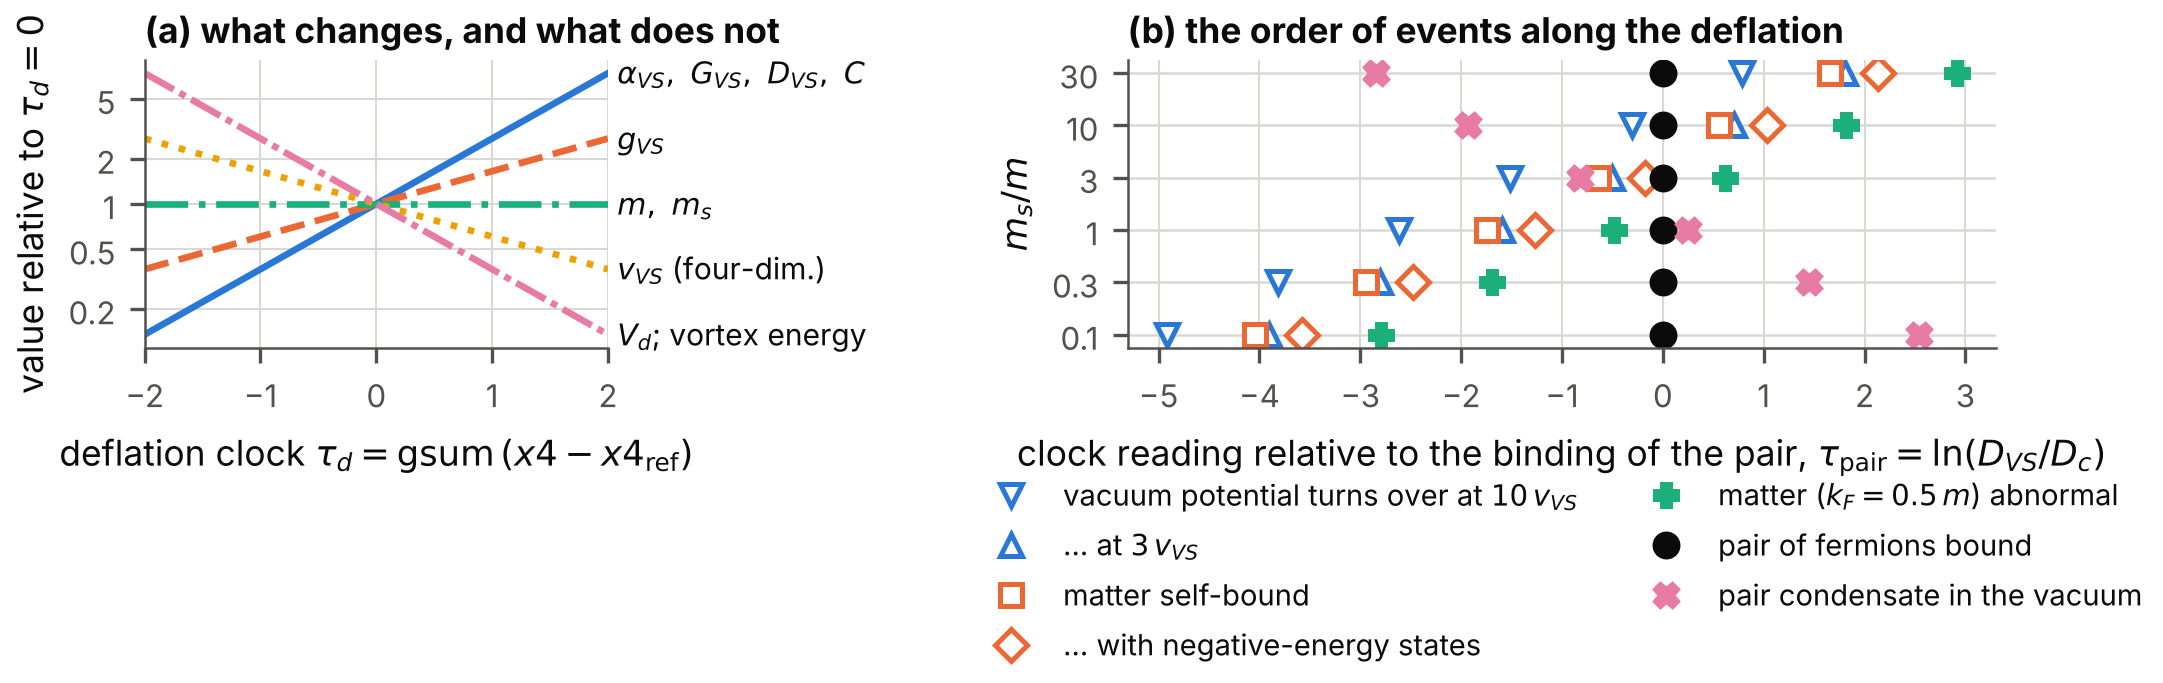
\includegraphics[width=1\textwidth,height=\textheight]{../figures/fig_clock.png}
\caption{The deflation clock. (a) How the quantities of the
four-dimensional description change with the clock \(\tau_d\)
(logarithmic scale; values relative to \(\tau_d=0\)). (b) The order of
events along the deflation for six ratios \(m_s/m\): clock reading of
each event relative to the moment at which two fermions form a bound
pair. Data: \texttt{data/coupling\_exponents.csv},
\texttt{data/events.csv}; programs: \texttt{deflation\ symmetry},
\texttt{deflation\ history}.}
\end{figure}

\begin{center}\rule{0.5\linewidth}{0.5pt}\end{center}

\hypertarget{the-modes-of-the-vorton-scalar-on-the-deflating-spacetimes}{%
\section{2. The modes of the Vorton-Scalar on the deflating
spacetimes}\label{the-modes-of-the-vorton-scalar-on-the-deflating-spacetimes}}

Write the Vorton-Scalar as in S1, Eq. (1.3), in terms of its
\textbf{radial mode} (a real field of mass \(m_s\)) and its
\textbf{phase mode} (a real massless field, the Goldstone boson of the
broken \(U(1)_{VS}\)). Let \(\varphi_{\rm bos}\) stand for either of
them, with the mass \(m_{\rm bos}=m_s\) or \(m_{\rm bos}=0\), and let
\(\hat\varphi_{\rm bos}=\sqrt{V_d}\,\varphi_{\rm bos}\) be its weighted
form. To first order in the field, its equation on the deflating
spacetime is
\[\frac{1}{V_d}\,\partial_4\big(V_d\,\partial_4\varphi_{\rm bos}\big)
+\Big(k^2+\eta_{44}\sum_t\frac{k_t^2}{b_t^2}+m_{\rm bos}^2\Big)\varphi_{\rm bos}=0,\tag{2.1}\]
for a mode with the wavenumber of magnitude \(k\) along the flat
coordinates and the wavenumbers \(k_t\) along the deflating ones. The
sign \(\eta_{44}\) is \(+1\) on 7+1 and \(-1\) on 4+4: on 4+4 the
deflating coordinates are time-like and their wavenumbers enter with the
opposite sign, as for the fermions.

\hypertarget{modes-that-do-not-depend-on-the-deflating-coordinates}{%
\subsection{2.1 Modes that do not depend on the deflating
coordinates}\label{modes-that-do-not-depend-on-the-deflating-coordinates}}

With \(k_t=0\), Eq. (2.1) reads
\(\varphi_{\rm bos}''-\mathrm{gsum}\,\varphi_{\rm bos}'+(k^2+m_{\rm bos}^2)\varphi_{\rm bos}=0\),
a linear equation with constant coefficients. Its solutions are
exponentials,
\[\varphi_{\rm bos}\ \propto\ \exp\Big\{\Big[\frac{\mathrm{gsum}}2\pm\sqrt{\frac{\mathrm{gsum}^2}{4}-k^2-m_{\rm bos}^2}\,\Big]\,x4\Big\}\tag{2.2}\]
(check \texttt{def-B2}). Define
\[\varpi_b=\sqrt{k^2+m_{\rm bos}^2-\frac{\mathrm{gsum}^2}{4}} .\]

\begin{itemize}
\tightlist
\item
  If \(k^2+m_{\rm bos}^2>\mathrm{gsum}^2/4\), the mode
  \textbf{oscillates} with the frequency \(\varpi_b\), and its amplitude
  grows as \(e^{\mathrm{gsum}\,x4/2}\). The growth is that of the weight
  alone: \(\hat\varphi_{\rm bos}\) has a constant amplitude. The number
  of quanta in a cell of fixed coordinates is conserved, and the cell
  shrinks.
\item
  If \(k^2+m_{\rm bos}^2<\mathrm{gsum}^2/4\), the mode \textbf{does not
  oscillate}. For the radial mode this never happens if
  \(m_s>\mathrm{gsum}/2\), which holds by many orders of magnitude for
  any rate of deflation that is not excluded by observation (RS3). For
  the phase mode it happens for \(k<\mathrm{gsum}/2\), that is, for
  wavelengths longer than \(4\pi/\mathrm{gsum}\).
\end{itemize}

\emph{What the non-oscillating phase modes mean.} At \(k=0\) the two
exponents are \(0\) and \(\mathrm{gsum}\). The first is a constant
phase, which costs nothing. The second is a phase that advances at a
rate proportional to \(1/V_d\): it is the conservation of the charge of
\(U(1)_{VS}\) in a shrinking volume. Neither is an instability of the
vacuum.

\hypertarget{the-field-of-a-static-source-the-potential-between-two-fermions}{%
\subsection{2.2 The field of a static source: the potential between two
fermions}\label{the-field-of-a-static-source-the-potential-between-two-fermions}}

Two fermions at rest attract each other by exchanging the radial mode.
On the deflating spacetime the density of a fixed number of fermions
grows as \(1/V_d\). The radial mode therefore obeys Eq. (2.1) with a
source proportional to \(e^{\mathrm{gsum}\,x4}\), and the solution that
follows the source is
\[\varphi_{\rm bos}=\frac{e^{\mathrm{gsum}\,x4}}{k^2+m_{\rm bos}^2}\times\text{(source)},\]
as substitution shows: the terms
\(\mathrm{gsum}^2-\mathrm{gsum}\cdot\mathrm{gsum}\) cancel. The
denominator contains the \emph{unshifted} mass. The potential between
two fermions at rest is therefore, at every moment, the Yukawa potential
of S1, \[V_s(r)=-\alpha_{VS}(x4)\,\frac{e^{-m_sr}}{r},\tag{2.3}\] with
the range \(1/m_s\) unchanged and the strength of the moment. The
numerical solution of Eq. (2.1) from rest approaches this form with a
transient that decays as \(e^{-\tau_d/2}\); after \(\tau_d=20\) the
relative difference is below \(4\times10^{-5}\) in the four cases
computed (check \texttt{def-B1}).

\begin{figure}
\centering
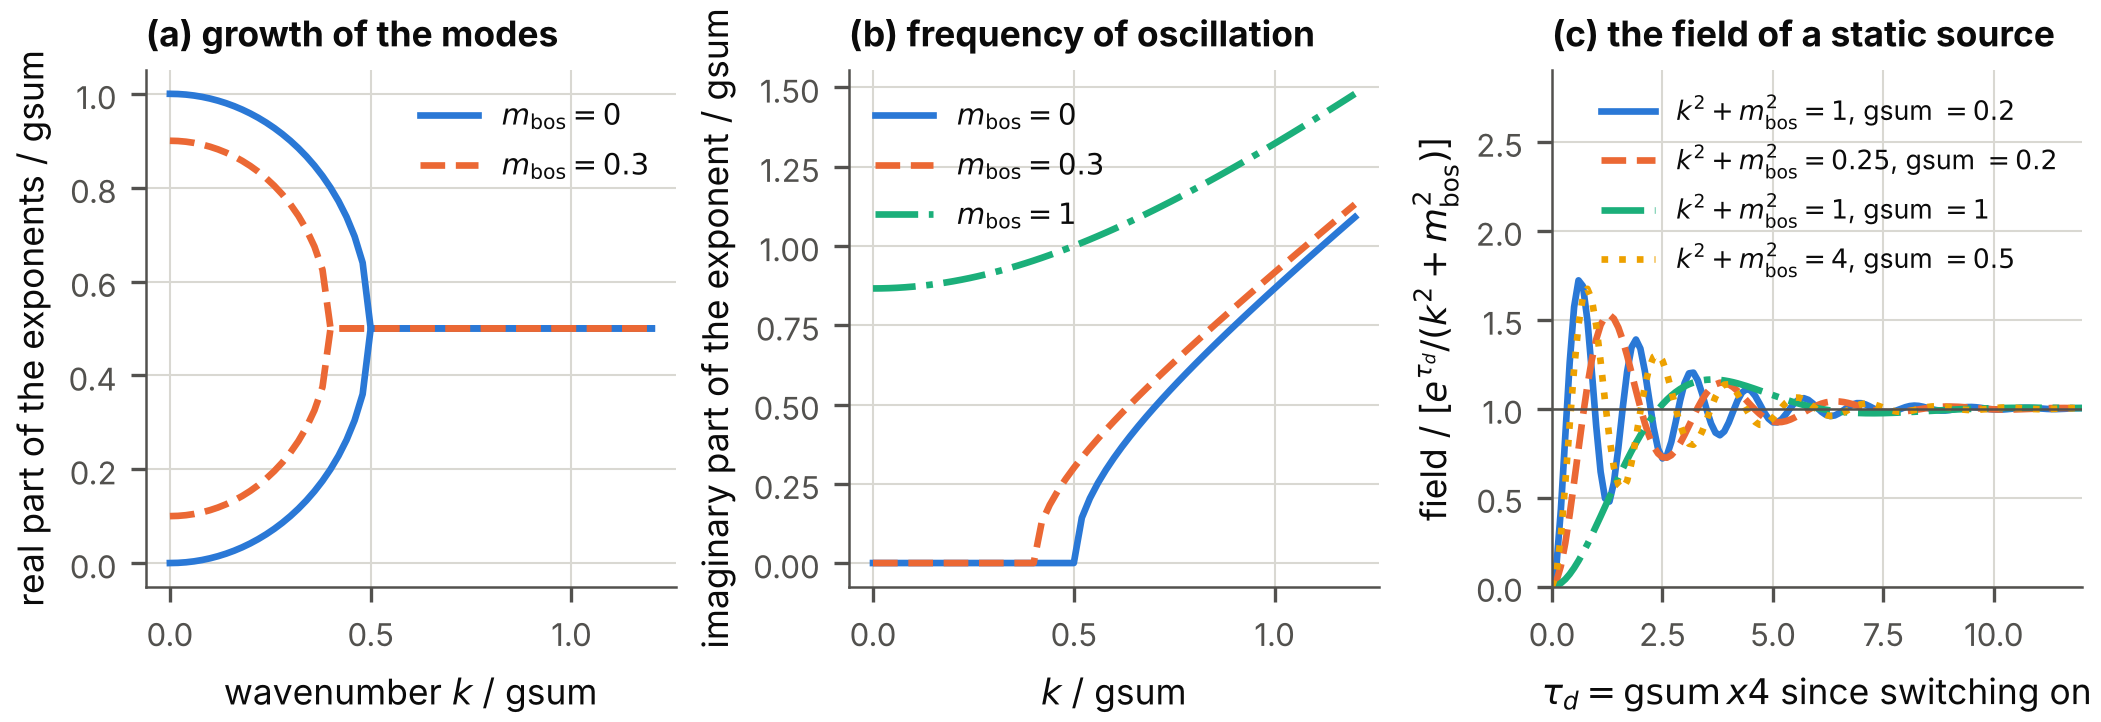
\includegraphics[width=1\textwidth,height=\textheight]{../figures/fig_scalar.png}
\caption{Modes of the Vorton-Scalar that do not depend on the deflating
coordinates. (a) Real parts of the two exponents of Eq. (2.2) against
the wavenumber, for the phase mode and for a radial mode, in units of
gsum. (b) Their imaginary part, the frequency of oscillation. (c) The
field that a static source builds up from zero, divided by the form
\(e^{\tau_d}/(k^2+m_{\rm bos}^2)\) that leads to Eq. (2.3). Data:
\texttt{data/scalar\_zero\_modes.csv}, \texttt{data/static\_source.csv};
program: \texttt{deflation\ channels}.}
\end{figure}

\hypertarget{modes-that-depend-on-a-deflating-coordinate}{%
\subsection{2.3 Modes that depend on a deflating
coordinate}\label{modes-that-depend-on-a-deflating-coordinate}}

For \(k_t\neq0\) the weighted field obeys
\(\hat\varphi_{\rm bos}''+\big(\varpi_b^2+\eta_{44}\,k_d(x4)^2\big)\hat\varphi_{\rm bos}=0\),
with the physical wavenumber \(k_d\) that grows exponentially. The two
spacetimes behave as they do for the fermions (DMD, Part 4).

\textbf{7+1: creation of quanta.} The frequency grows without bound.
When one rate governs, the solutions are Bessel functions of the
imaginary order \(i\varpi_b/\mathrm{rate}_t\) and of the argument
\(u_d\), and a mode that starts empty ends with
\[n_{\rm cr}=\frac{1}{e^{2\pi\varpi_b/\mathrm{rate}_t}-1}\tag{2.4}\]
quanta: the Bose--Einstein distribution at the temperature
\(T_{\rm defl}=\mathrm{rate}_t/2\pi\), the same temperature as for the
fermions. The program confirms Eq. (2.4) in 36 cases to a relative
deviation of \(1.9\times10^{-5}\) (check \texttt{def-B3}; independently
\texttt{Idef-B1}). The figure of DMD, Sec. 4.2, shows both laws.

\textbf{4+4: extinction.} Beyond the turning value at which
\(k_d=\varpi_b\) one solution decays and one grows. The bounded solution
is the modified Bessel function of the order
\(i\varpi_b/\mathrm{rate}_t\) that decays at large argument. At early
times it is a standing wave; at late times it falls as \(e^{-u_d}\)
(check \texttt{def-B4}). The scalar field, like the fermion field, loses
its dependence on the deflating times.

\begin{center}\rule{0.5\linewidth}{0.5pt}\end{center}

\hypertarget{the-pairing-interaction-and-the-gap-along-the-clock}{%
\section{3. The pairing interaction and the gap along the
clock}\label{the-pairing-interaction-and-the-gap-along-the-clock}}

\hypertarget{exchange-amplitudes}{%
\subsection{3.1 Exchange amplitudes}\label{exchange-amplitudes}}

S1, Sec. 4, defines for every pair channel the exchange amplitudes
\(F_S\) and \(F_P\) of the radial mode and of the phase mode: the matrix
elements of the one-boson exchange between two fermions of opposite
momenta in the internal state of the channel. They are computed from the
Dirac matrices of the frame, which the deflation does not change, and
each is proportional to the square of the coupling. Therefore, for
fields that do not depend on \(x5,x6,x7\),
\[F_{S,P}\ \text{on the deflating spacetime at the time }x4\;=\;g_{VS}(x4)^2\times\big(F_{S,P}\ \text{of S1 at }g_{VS}=1\big).\tag{3.1}\]
The program computes the amplitudes of all 90 pair channels again, from
the matrices of each deflating spacetime, and compares them with the
file of the main project: the 1170 rows agree to the digits printed
there (check \texttt{def-K1}), and the amplitudes of the hidden-axis
channel reproduce the closed forms of S1 to \(1.1\times10^{-15}\) (check
\texttt{def-K2}).

The conclusion of S1 about the channels therefore stands at every
moment: the radial mode attracts in every channel; the phase mode
attracts in the \textbf{vector pairs along the extra axes} and repels in
their two-form partners; the most attractive channel is the vector pair
along an extra axis, the \emph{hidden-axis singlet}.

\begin{figure}
\centering
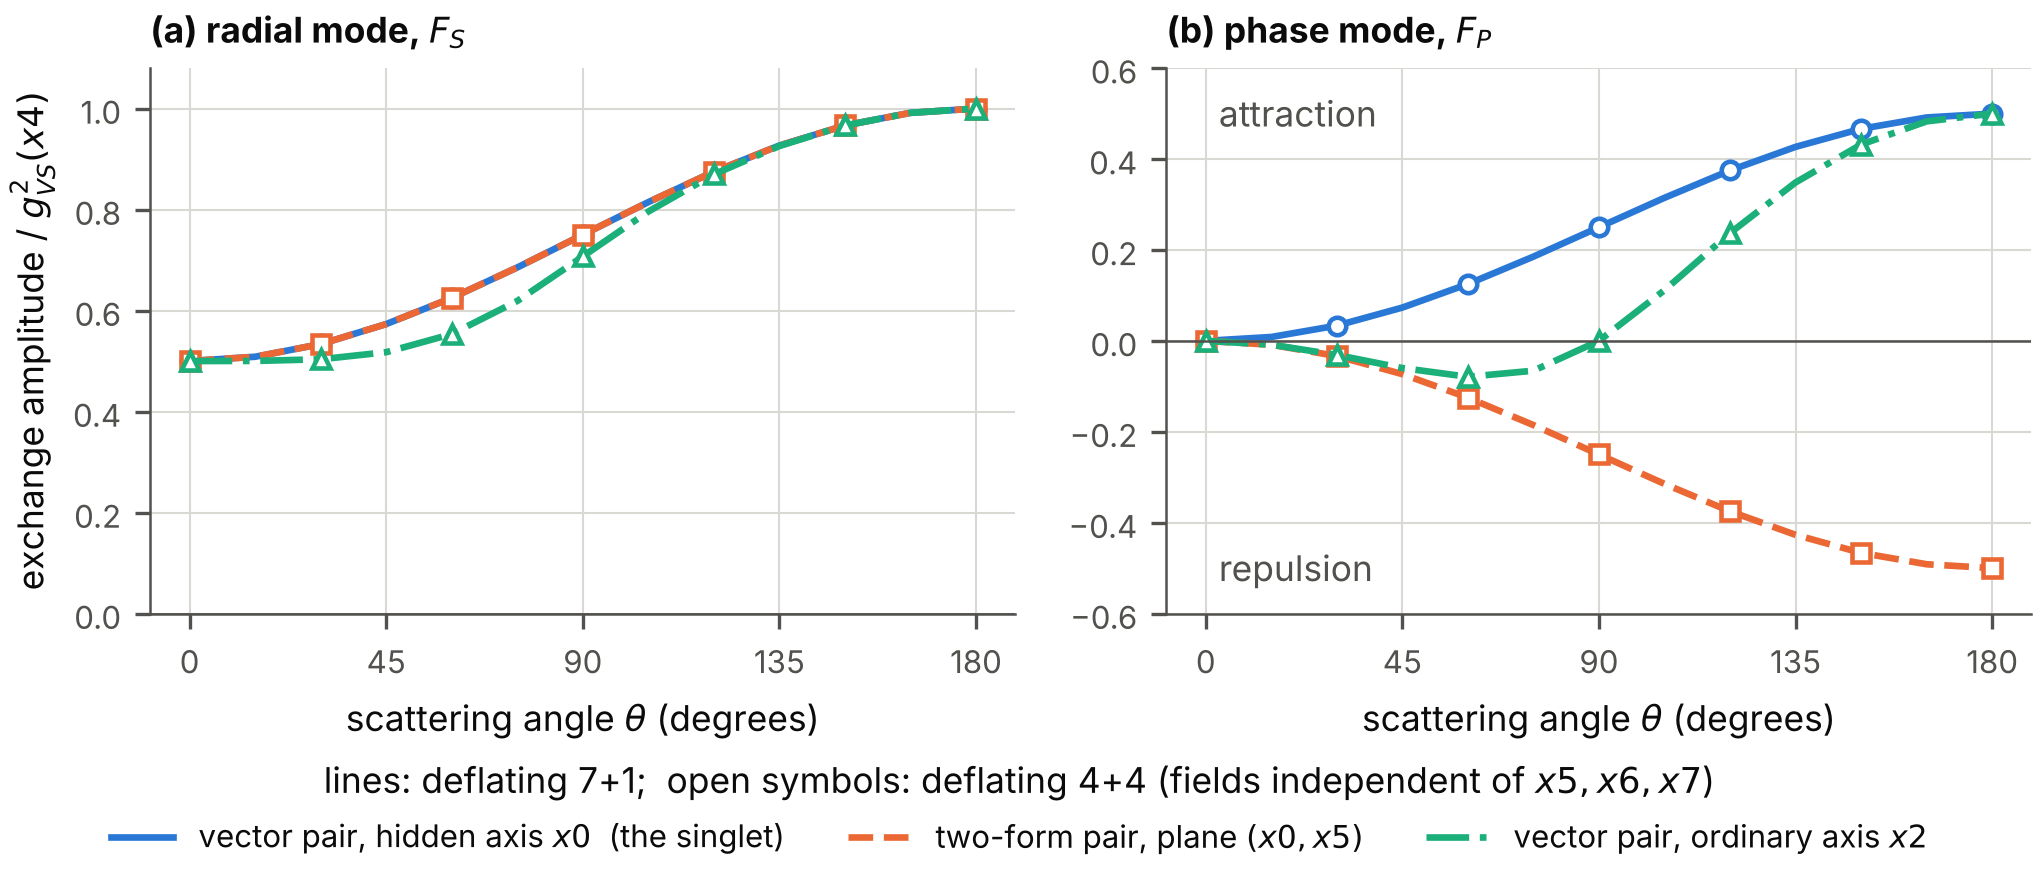
\includegraphics[width=1\textwidth,height=\textheight]{../figures/fig_kernels.png}
\caption{Exchange amplitudes in three pair channels, divided by the
square of the coupling of the moment, against the scattering angle.
Lines: 7+1; open symbols: 4+4. The amplitudes are those of the main
project: the deflation changes their overall strength and nothing else.
Data: \texttt{data/pair\_channel\_kernel.csv}; program:
\texttt{deflation\ channels}.}
\end{figure}

\hypertarget{the-gap-grows-and-much-faster-than-the-coupling}{%
\subsection{3.2 The gap grows, and much faster than the
coupling}\label{the-gap-grows-and-much-faster-than-the-coupling}}

The gap equation of S1, Sec. 5, holds at each moment with the couplings
of that moment. Its solution as a function of the clock is the
\textbf{adiabatic history} of the paired state: the state that matter of
a given density would have if it were always in equilibrium. (Section 7
examines when it can be.) The program solves the gap equation at 34
moments for each of four sets of the mass \(m_s\) and the Fermi momentum
\(k_F\). Recall the dimensionless pairing strength
\(\lambda=N(0)\,W(k_F,k_F)\) of S1 (density of states at the Fermi
surface times the kernel of the gap equation there); in the vector
channel it is the sum \(\lambda_S+\lambda_P\) of the contributions of
the two modes.

\begin{longtable}[]{@{}
  >{\raggedright\arraybackslash}p{(\columnwidth - 14\tabcolsep) * \real{0.1250}}
  >{\raggedleft\arraybackslash}p{(\columnwidth - 14\tabcolsep) * \real{0.1250}}
  >{\raggedleft\arraybackslash}p{(\columnwidth - 14\tabcolsep) * \real{0.1250}}
  >{\raggedleft\arraybackslash}p{(\columnwidth - 14\tabcolsep) * \real{0.1250}}
  >{\raggedleft\arraybackslash}p{(\columnwidth - 14\tabcolsep) * \real{0.1250}}
  >{\raggedleft\arraybackslash}p{(\columnwidth - 14\tabcolsep) * \real{0.1250}}
  >{\raggedleft\arraybackslash}p{(\columnwidth - 14\tabcolsep) * \real{0.1250}}
  >{\raggedleft\arraybackslash}p{(\columnwidth - 14\tabcolsep) * \real{0.1250}}@{}}
\toprule\noalign{}
\begin{minipage}[b]{\linewidth}\raggedright
\(m_s/m\), \(k_F/m\)
\end{minipage} & \begin{minipage}[b]{\linewidth}\raggedleft
\(\tau_d\)
\end{minipage} & \begin{minipage}[b]{\linewidth}\raggedleft
\(g_{VS}\)
\end{minipage} & \begin{minipage}[b]{\linewidth}\raggedleft
\(\lambda\)
\end{minipage} & \begin{minipage}[b]{\linewidth}\raggedleft
gap\(/E_F\)
\end{minipage} & \begin{minipage}[b]{\linewidth}\raggedleft
\(T_c/\)gap
\end{minipage} & \begin{minipage}[b]{\linewidth}\raggedleft
rate of growth
\end{minipage} & \begin{minipage}[b]{\linewidth}\raggedleft
\(\lambda\,\times\) rate
\end{minipage} \\
\midrule\noalign{}
\endhead
\bottomrule\noalign{}
\endlastfoot
0.10, 0.50 & -0.63 & 0.730 & 0.062 & \(1.17\times10^{-7}\) & 0.567 & ---
& --- \\
0.10, 0.50 & -0.13 & 0.939 & 0.102 & \(7.40\times10^{-5}\) & 0.567 &
9.88 & 1.01 \\
0.10, 0.50 & 0.38 & 1.208 & 0.169 & \(3.70\times10^{-3}\) & 0.567 & 6.01
& 1.01 \\
0.10, 0.50 & 0.88 & 1.554 & 0.279 & 0.0407 & 0.565 & 3.74 & --- \\
0.10, 0.50 & 1.39 & 2.000 & 0.463 & 0.189 & 0.555 & 2.50 & --- \\
0.10, 0.50 & 1.89 & 2.573 & 0.766 & 0.563 & 0.528 & 1.96 & --- \\
0.10, 0.50 & 2.39 & 3.311 & 1.268 & 1.49 & 0.480 & 1.96 & --- \\
1.0, 0.50 & 0.88 & 1.554 & 0.056 & \(1.02\times10^{-7}\) & 0.567 & --- &
--- \\
1.0, 0.50 & 1.13 & 1.763 & 0.072 & \(5.62\times10^{-6}\) & 0.567 & 14.02
& 1.01 \\
1.0, 0.50 & 1.39 & 2.000 & 0.092 & \(1.27\times10^{-4}\) & 0.567 & 10.93
& 1.01 \\
1.0, 0.50 & 1.64 & 2.269 & 0.119 & \(1.45\times10^{-3}\) & 0.567 & 8.54
& 1.02 \\
1.0, 0.50 & 1.89 & 2.573 & 0.153 & \(9.76\times10^{-3}\) & 0.567 & 6.71
& 1.03 \\
1.0, 0.50 & 2.14 & 2.919 & 0.197 & 0.0439 & 0.566 & 5.33 & --- \\
1.0, 0.50 & 2.39 & 3.311 & 0.253 & 0.147 & 0.563 & 4.37 & --- \\
\end{longtable}

(The rate of growth in the last two columns is
\(d\ln(\mathrm{gap})/d\tau_d\); the last column is given where the gap
is between \(10^{-6}\) and \(0.02\) of \(E_F\).) Three results (checks
\texttt{def-H2}, \texttt{def-H3}):

\begin{enumerate}
\def\labelenumi{\arabic{enumi}.}
\tightlist
\item
  \emph{The order of the channels does not change.} At every moment the
  gap of the vector channel is at least as large as the gap with the
  radial mode alone, and that at least as large as the gap of the
  two-form channel. The gap never decreases.
\item
  \emph{The critical temperature follows the gap.} Wherever the gap is
  below 5 per cent of the Fermi kinetic energy \(E_F\), the critical
  temperature is \(T_c=0.567\) times the gap, the weak-coupling ratio,
  to within 0.002.
\item
  \emph{The law of growth.} In weak coupling the gap is proportional to
  \(e^{-1/\lambda}\), and \(\lambda\propto e^{\tau_d}\). Hence
  \[\frac{d\ln(\mathrm{gap})}{d\tau_d}=\frac1\lambda .\tag{3.2}\] In the
  computed histories the product \(\lambda\,d\ln(\mathrm{gap})/d\tau_d\)
  lies between 1.00 and 1.03 wherever the gap is between \(10^{-6}\) and
  \(0.02\) of \(E_F\).
\end{enumerate}

Equation (3.2) is the central quantitative statement of this supplement.
While the coupling grows by one e-folding, the gap of a weakly paired
state with \(\lambda=0.1\) grows by ten e-foldings, a factor of twenty
thousand. A paired state that is unobservably weak at one time becomes
strong within a few e-foldings of the volume.

\begin{figure}
\centering
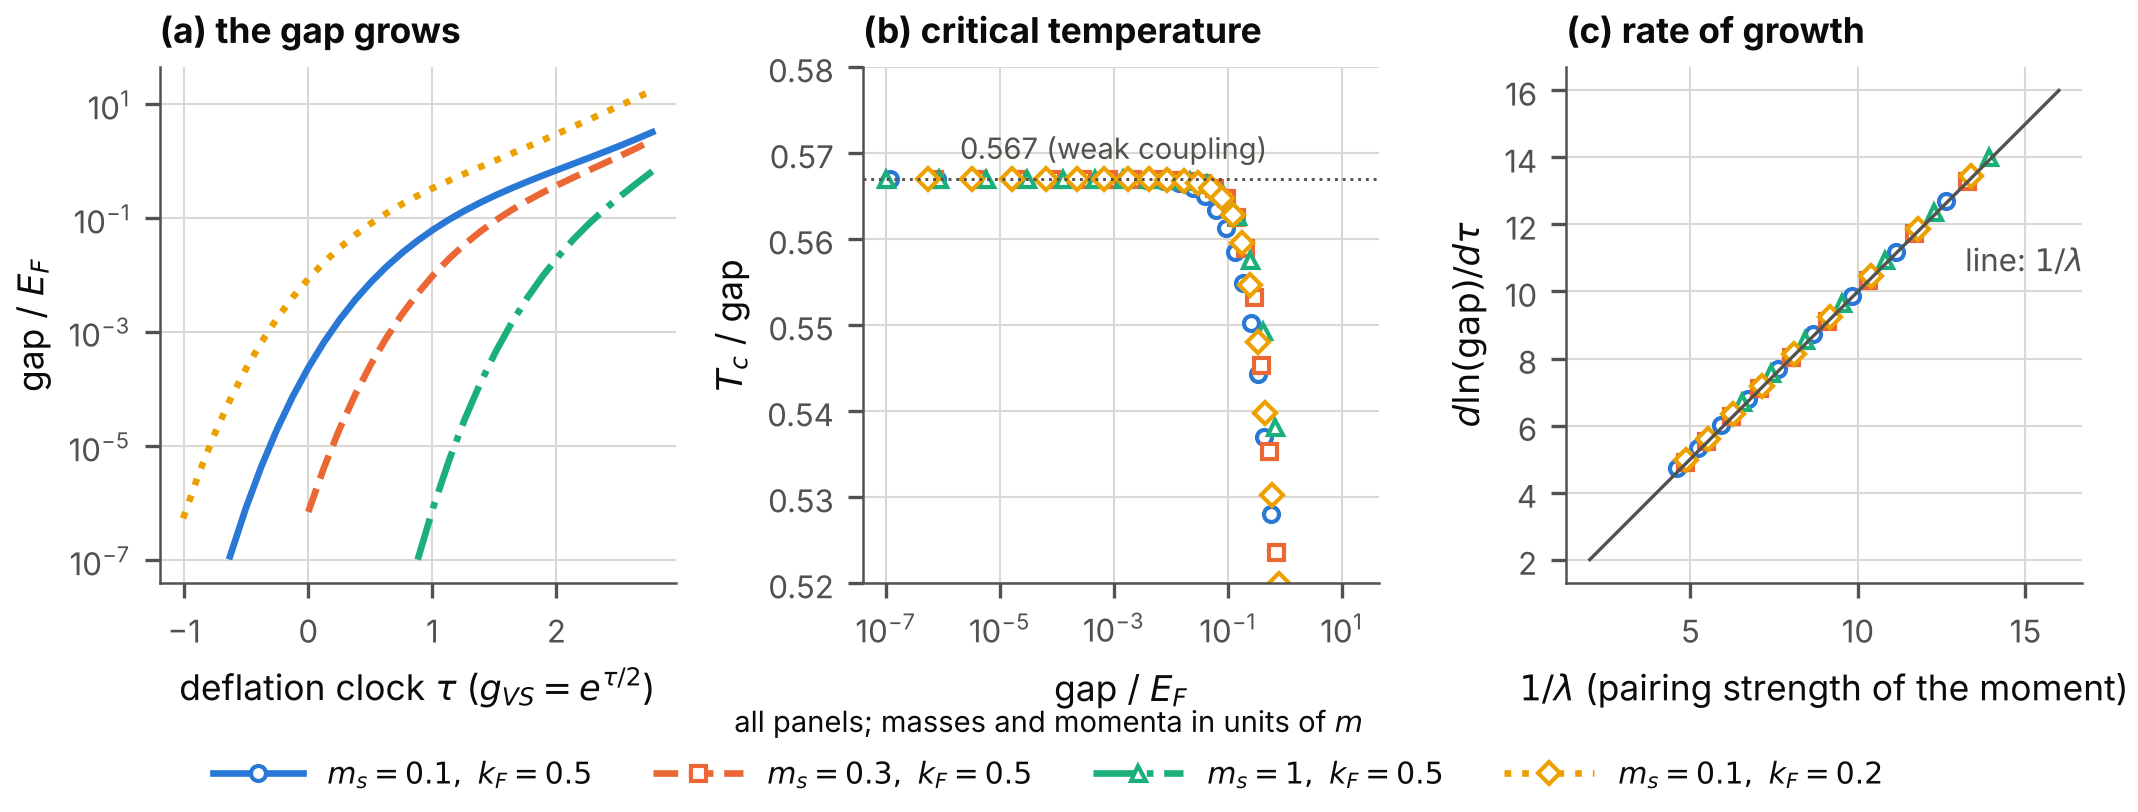
\includegraphics[width=1\textwidth,height=\textheight]{../figures/fig_gap_history.png}
\caption{The gap along the deflation clock, for four sets of the mass of
the radial mode and of the Fermi momentum (units of \(m\)). (a) The gap
of the vector channel in units of the Fermi kinetic energy. (b) The
ratio of the critical temperature to the gap. (c) The rate of growth of
the gap against \(1/\lambda\); the line is Eq. (3.2). Data:
\texttt{data/gap\_history.csv}; program: \texttt{deflation\ history}.}
\end{figure}

\begin{center}\rule{0.5\linewidth}{0.5pt}\end{center}

\hypertarget{the-bound-pair}{%
\section{4. The bound pair}\label{the-bound-pair}}

\hypertarget{the-moment-of-binding}{%
\subsection{4.1 The moment of binding}\label{the-moment-of-binding}}

Two fermions in the Yukawa potential (2.3) form a bound state if and
only if \(D_{VS}=\alpha_{VS}\,m/m_s\) exceeds the critical value
\(D_c=1.67981\) (S1, Sec. 5.3; check \texttt{def-H1}). On a deflating
spacetime \(D_{VS}\propto e^{\tau_d}\), so the pair becomes bound at a
definite time. Measure the clock from that moment:
\[\tau_{\rm pair}=\ln\frac{D_{VS}}{D_c}=\mathrm{gsum}\,\big(x4-x4_{\rm binding}\big).\tag{4.1}\]

\begin{longtable}[]{@{}
  >{\raggedleft\arraybackslash}p{(\columnwidth - 8\tabcolsep) * \real{0.2000}}
  >{\raggedleft\arraybackslash}p{(\columnwidth - 8\tabcolsep) * \real{0.2000}}
  >{\raggedleft\arraybackslash}p{(\columnwidth - 8\tabcolsep) * \real{0.2000}}
  >{\raggedleft\arraybackslash}p{(\columnwidth - 8\tabcolsep) * \real{0.2000}}
  >{\raggedleft\arraybackslash}p{(\columnwidth - 8\tabcolsep) * \real{0.2000}}@{}}
\toprule\noalign{}
\begin{minipage}[b]{\linewidth}\raggedleft
\(\tau_{\rm pair}\)
\end{minipage} & \begin{minipage}[b]{\linewidth}\raggedleft
\(D_{VS}\)
\end{minipage} & \begin{minipage}[b]{\linewidth}\raggedleft
scattering length \(\times\,m_s\)
\end{minipage} & \begin{minipage}[b]{\linewidth}\raggedleft
bound states
\end{minipage} & \begin{minipage}[b]{\linewidth}\raggedleft
\(E_b\times m/m_s^2\)
\end{minipage} \\
\midrule\noalign{}
\endhead
\bottomrule\noalign{}
\endlastfoot
-0.105 & 1.5118 & -12.50 & 0 & 0 \\
-0.095 & 1.5279 & -13.93 & 0 & 0 \\
-0.010 & 1.6630 & -134.0 & 0 & 0 \\
0.010 & 1.6966 & 135.9 & 1 & \(5.50\times10^{-5}\) \\
0.486 & 2.7314 & 2.698 & 1 & 0.232 \\
0.994 & 4.5409 & -0.1288 & 1 & 1.82 \\
\end{longtable}

\emph{The scattering length.} Just before the binding the scattering
length \(a_{\rm sc}\) of two fermions is large and negative, just after
it large and positive: \(-134.0/m_s\) at \(0.99\,D_c\) and
\(+135.9/m_s\) at \(1.01\,D_c\) (check \texttt{def-H4}). At the moment
of binding it is infinite: the two fermions are at a scattering
resonance. Every pair of fermions of the model passes through this
resonance once, at the same time. The supplement RS3 examines what that
means if the fermions are the dark matter.

\emph{The binding energy.} Just after the binding the binding energy
starts quadratically,
\[E_b\ \propto\ \big(e^{\tau_{\rm pair}}-1\big)^2\,\frac{m_s^2}{m},\tag{4.2}\]
with the fitted exponents 2.01 between 2 and 4 per cent and between 4
and 8 per cent above \(D_c\). Because \(E_b\) vanishes at the threshold,
the time \(1/E_b\) that the pair needs to adjust is infinite there.
\emph{However slow the deflation is, the pair cannot follow it
adiabatically at first.}

\emph{From the gap equation.} The same threshold appears in the gap
equation of the paired state in vacuum, whose kernel is relativistic:
its linearized form reaches the eigenvalue 1 at \(D_{VS}=1.7347\),
\(1.6902\), \(1.6810\) for \(m_s/m=0.3\), \(0.1\), \(0.03\), approaching
1.67981 as the binding becomes non-relativistic (check \texttt{def-P6}
of the supplement RS4).

\begin{figure}
\centering
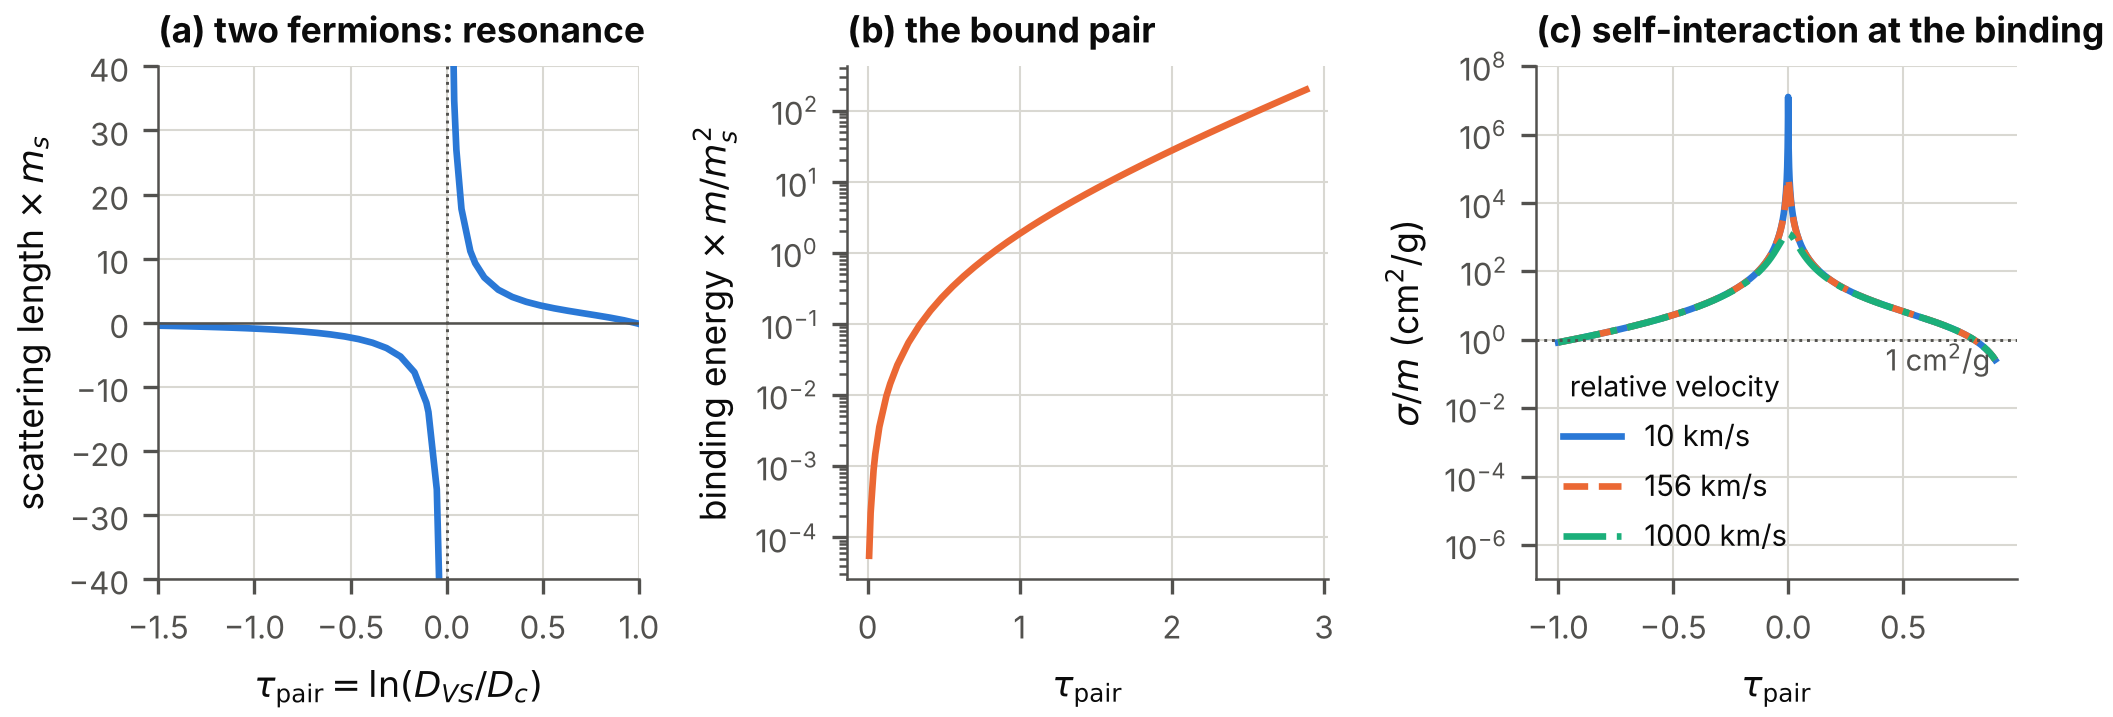
\includegraphics[width=1\textwidth,height=\textheight]{../figures/fig_binding.png}
\caption{The bound pair along the clock. (a) Scattering length of two
fermions in units of \(1/m_s\) against \(\tau_{\rm pair}\): the
resonance at the moment of binding. (b) Binding energy of the pair. (c)
Cross-section per mass of two fermions at three relative velocities
while the clock passes the binding (supplement RS3). Data:
\texttt{data/dimer\_history.csv}, \texttt{data/dm\_resonance.csv};
programs: \texttt{deflation\ history}, \texttt{deflation\ matter}.}
\end{figure}

\hypertarget{the-order-of-events}{%
\subsection{4.2 The order of events}\label{the-order-of-events}}

The other thresholds of the main project are thresholds in
\(C=g_{VS}^2m^2/m_s^2\), which grows at the same rate as \(D_{VS}\).
With \(C/D_{VS}=4\pi m/m_s\) fixed, the order in which the events happen
depends on the ratio \(m_s/m\) alone. The table gives the clock reading
\(\tau_{\rm pair}\) of each event; a negative number means that the
event precedes the binding of the pair.

\begin{longtable}[]{@{}
  >{\raggedright\arraybackslash}p{(\columnwidth - 14\tabcolsep) * \real{0.2619}}
  >{\raggedright\arraybackslash}p{(\columnwidth - 14\tabcolsep) * \real{0.1667}}
  >{\raggedleft\arraybackslash}p{(\columnwidth - 14\tabcolsep) * \real{0.0952}}
  >{\raggedleft\arraybackslash}p{(\columnwidth - 14\tabcolsep) * \real{0.0952}}
  >{\raggedleft\arraybackslash}p{(\columnwidth - 14\tabcolsep) * \real{0.0952}}
  >{\raggedleft\arraybackslash}p{(\columnwidth - 14\tabcolsep) * \real{0.0952}}
  >{\raggedleft\arraybackslash}p{(\columnwidth - 14\tabcolsep) * \real{0.0952}}
  >{\raggedleft\arraybackslash}p{(\columnwidth - 14\tabcolsep) * \real{0.0952}}@{}}
\toprule\noalign{}
\begin{minipage}[b]{\linewidth}\raggedright
event
\end{minipage} & \begin{minipage}[b]{\linewidth}\raggedright
threshold
\end{minipage} & \begin{minipage}[b]{\linewidth}\raggedleft
\(m_s/m=0.1\)
\end{minipage} & \begin{minipage}[b]{\linewidth}\raggedleft
\(m_s/m=0.3\)
\end{minipage} & \begin{minipage}[b]{\linewidth}\raggedleft
\(m_s/m=1\)
\end{minipage} & \begin{minipage}[b]{\linewidth}\raggedleft
\(m_s/m=3\)
\end{minipage} & \begin{minipage}[b]{\linewidth}\raggedleft
\(m_s/m=10\)
\end{minipage} & \begin{minipage}[b]{\linewidth}\raggedleft
\(m_s/m=30\)
\end{minipage} \\
\midrule\noalign{}
\endhead
\bottomrule\noalign{}
\endlastfoot
the one-loop potential of the Vorton-Scalar falls below its vacuum value
at the field \(10\,v_{VS}\) & \(C=1.5477\) & -4.92 & -3.82 & -2.61 &
-1.51 & -0.31 & 0.79 \\
matter is self-bound (Fermi sea only) & \(C=3.7011\) & -4.04 & -2.94 &
-1.74 & -0.64 & 0.56 & 1.66 \\
the one-loop potential falls below its vacuum value at the field
\(3\,v_{VS}\) & \(C=4.2694\) & -3.90 & -2.80 & -1.60 & -0.50 & 0.70 &
1.80 \\
matter is self-bound (with the negative-energy states) & \(C=5.9218\) &
-3.57 & -2.48 & -1.27 & -0.17 & 1.03 & 2.13 \\
matter of Fermi momentum \(0.5\,m\) becomes abnormal (massless fermions)
& \(C=12.9713\) & -2.79 & -1.69 & -0.49 & 0.61 & 1.82 & 2.91 \\
\textbf{two fermions form a bound pair} & \(D_{VS}=1.6798\) & 0.00 &
0.00 & 0.00 & 0.00 & 0.00 & 0.00 \\
pair condensate in the vacuum (ladder equation, cutoff \(100\,m\)) &
\(\alpha_{VS}=2.13\) to \(2.93\) & 2.54 & 1.44 & 0.25 & -0.82 & -1.93 &
-2.84 \\
\end{longtable}

The events other than the binding are derived in the supplement RS4. The
table shows (check \texttt{def-H8}):

\begin{itemize}
\tightlist
\item
  For a \textbf{light radial mode} (\(m_s/m\le3\) in the table) the pair
  becomes bound only \emph{after} the one-loop potential of the
  Vorton-Scalar has fallen below its vacuum value at a field of three
  times the vacuum value: the deflation endangers the vacuum of the
  model before it binds the pair. The condition for the opposite order
  is \(4\pi D_c\,m/m_s<4.27\), that is \(m_s/m>4.9\).
\item
  For a \textbf{heavy radial mode} (\(m_s/m=10\), \(30\)) the pair
  becomes bound first, and matter becomes self-bound and abnormal later.
\end{itemize}

Which of the two orders nature would have chosen is not decided by
anything in the model; the table states what follows from each choice.

\begin{center}\rule{0.5\linewidth}{0.5pt}\end{center}

\hypertarget{the-order-parameter-and-the-ground-state}{%
\section{5. The order parameter and the ground
state}\label{the-order-parameter-and-the-ground-state}}

\hypertarget{frame-components-and-coordinate-components}{%
\subsection{5.1 Frame components and coordinate
components}\label{frame-components-and-coordinate-components}}

The order parameter of S1 is the expectation value \(\Delta^a\) of the
vector pair operator along the extra axis \(a\in\{0,5,6,7\}\): four
complex numbers. On the deflating spacetimes the index \(a\) is a
\emph{frame} index: \(\Delta^a\) is the component along the unit vector
\(e_a\). The coordinate components along the deflating coordinates are
\(\Delta_t=b_t(x4)\,\Delta^t\) and shrink with the scale factors when
the frame components are constant. All statements below are about frame
components.

\emph{The quartic invariant.} The energy of S1 depends on the order
parameter through the \(8\times8\) gap matrix \(\mathsf M\) on the
internal states of a pair. The identity
\[\tfrac18\,\mathrm{Tr}\big[(\mathsf M\mathsf M^\dagger)^2\big]
=2\Big(\sum_a\lvert\Delta^a\rvert^2\Big)^2-\Big\lvert\sum_{a,b}\eta_{ab}\,\Delta^a\Delta^b\Big\rvert^2\tag{5.1}\]
holds on both deflating spacetimes with the frame metric \(\eta_{ab}\)
of the four axes (check \texttt{def-K3}, to \(2\times10^{-14}\)). In
coordinate components the same expression contains the metric \(g_{tt}\)
of the moment.

\hypertarget{the-ground-state-no-direction-is-preferred}{%
\subsection{5.2 The ground state: no direction is
preferred}\label{the-ground-state-no-direction-is-preferred}}

The potential of the paired state as a function of the order parameter
is computed in the supplement RS4. Its result for the six states
examined on each spacetime:

\begin{longtable}[]{@{}
  >{\raggedright\arraybackslash}p{(\columnwidth - 12\tabcolsep) * \real{0.1143}}
  >{\raggedright\arraybackslash}p{(\columnwidth - 12\tabcolsep) * \real{0.3143}}
  >{\raggedleft\arraybackslash}p{(\columnwidth - 12\tabcolsep) * \real{0.1143}}
  >{\raggedleft\arraybackslash}p{(\columnwidth - 12\tabcolsep) * \real{0.1143}}
  >{\raggedleft\arraybackslash}p{(\columnwidth - 12\tabcolsep) * \real{0.1143}}
  >{\raggedleft\arraybackslash}p{(\columnwidth - 12\tabcolsep) * \real{0.1143}}
  >{\raggedleft\arraybackslash}p{(\columnwidth - 12\tabcolsep) * \real{0.1143}}@{}}
\toprule\noalign{}
\begin{minipage}[b]{\linewidth}\raggedright
spacetime
\end{minipage} & \begin{minipage}[b]{\linewidth}\raggedright
state
\end{minipage} & \begin{minipage}[b]{\linewidth}\raggedleft
smaller gap\(^2\)
\end{minipage} & \begin{minipage}[b]{\linewidth}\raggedleft
larger gap\(^2\)
\end{minipage} & \begin{minipage}[b]{\linewidth}\raggedleft
potential
\end{minipage} & \begin{minipage}[b]{\linewidth}\raggedleft
flat directions
\end{minipage} & \begin{minipage}[b]{\linewidth}\raggedleft
positive directions
\end{minipage} \\
\midrule\noalign{}
\endhead
\bottomrule\noalign{}
\endlastfoot
7+1 & pair along the frame axis of \(x0\) (hidden-axis singlet) & 1.000
& 1.000 & -2.0000 & 4 & 4 \\
7+1 & pair along the frame axis of \(x5\) & 1.000 & 1.000 & -2.0000 & 4
& 4 \\
7+1 & pair along the frame axis of \(x7\) & 1.000 & 1.000 & -2.0000 & 4
& 4 \\
7+1 & unitary, rotated between \(x0\) and \(x5\) & 1.000 & 1.000 &
-2.0000 & 4 & 4 \\
7+1 & unitary, general direction and phase & 1.000 & 1.000 & -2.0000 & 4
& 4 \\
7+1 & half-paired: \(\eta_{ab}\Delta^a\Delta^b=0\) & 0.000 & 1.000 &
-1.0000 & --- & --- \\
4+4 & pair along the frame axis of \(x0\) (hidden-axis singlet) & 1.000
& 1.000 & -2.0000 & 4 & 4 \\
4+4 & pair along the frame axis of \(x5\) & 1.000 & 1.000 & -2.0000 & 4
& 4 \\
4+4 & pair along the frame axis of \(x7\) & 1.000 & 1.000 & -2.0000 & 4
& 4 \\
4+4 & unitary, rotated between \(x0\) and \(x5\) & 1.000 & 1.000 &
-2.0000 & 4 & 4 \\
4+4 & unitary, general direction and phase & 1.000 & 1.000 & -2.0000 & 4
& 4 \\
4+4 & half-paired: \(\eta_{ab}\Delta^a\Delta^b=0\) & 0.000 & 1.000 &
-1.0000 & --- & --- \\
\end{longtable}

Every \textbf{unitary} state --- a state in which \(\Delta^a\) is a real
unit vector times a phase --- has all eight gaps equal and the lowest
potential, whichever direction the vector has. It has four flat
directions (the Goldstone modes: one phase and three rotations of the
direction) and four directions of positive curvature. The
\textbf{half-paired} states, in which four of the eight gaps vanish,
have half the condensation energy. The potential does not distinguish
the deflating axes from \(x0\) (check \texttt{def-P4}).

\emph{What this means.} One might have expected the deflation to select
the direction of the order parameter: the hidden axis \(x0\), which does
not deflate, against the three that do. In the sector of fields that do
not depend on the extra coordinates it does not. The reason is the
central observation of DMD: in this sector the weighted field obeys the
flat equations, whose internal symmetry \(SU(2)_A\times SU(2)_B\)
rotates the four frame axes into one another (check \texttt{def-S3}).
The symmetry of the ground-state manifold is larger than the symmetry of
the spacetime. The supplement RS2 takes up the consequences.

\begin{center}\rule{0.5\linewidth}{0.5pt}\end{center}

\hypertarget{vortices-and-their-zero-modes}{%
\section{6. Vortices and their zero
modes}\label{vortices-and-their-zero-modes}}

\hypertarget{the-vortex-line-of-the-vorton-scalar}{%
\subsection{6.1 The vortex line of the
Vorton-Scalar}\label{the-vortex-line-of-the-vorton-scalar}}

Because the vacuum value of the Vorton-Scalar breaks the phase symmetry
\(U(1)_{VS}\), the field has line-like defects (S1, Sec. 8): along a
straight line, say the \(x3\) axis, its magnitude vanishes, and around
the line its phase winds by \(2\pi\) times an integer. For unit winding,
\(\Phi_{VS}=(v_{VS}/\sqrt2)\,\times\) (a profile that rises from 0 on
the line to 1 at a distance of order \(1/m_s\))
\(\times\,e^{i\theta_{12}}\), with \(\theta_{12}\) the angle around the
line in the plane of \(x1\) and \(x2\).

\emph{Energy per unit length.} It is proportional to the square of the
four-dimensional vacuum value, and so falls as \(e^{-\tau_d}\): in the
four-dimensional description \textbf{vortex lines become lighter as the
deflation proceeds}, while their core, of radius \(1/m_s\), keeps its
size.

\hypertarget{fermions-on-the-line-four-zero-modes-for-unit-winding}{%
\subsection{6.2 Fermions on the line: four zero modes for unit
winding}\label{fermions-on-the-line-four-zero-modes-for-unit-winding}}

On the line the fermion mass \(m=g_{VS}\times\) (magnitude of the field)
vanishes, and fermions can be trapped there. With
\(\Phi P^R+\Phi^*P^L=\lvert\Phi\rvert\,e^{i\chi\arg\Phi}\) the
Hamiltonian of a fermion in the field of the vortex is
\[\sum_{j=1}^3\alpha^j\,p_j+m\,(\text{profile})\,\beta\,\big(\cos\theta_{12}+i\chi\,\sin\theta_{12}\big),\]
with the matrices \(\alpha^j\), \(\beta\) and the chirality matrix
\(\chi\) of the spacetime at hand, and the momenta \(p_j\) along
\(x1,x2,x3\). A state of zero energy at zero momentum along the line has
the form of a constant spinor \(w_z\) times a function that decays away
from the line as \(\exp(-m\int\text{profile})\). Inserting this form,
the Hamiltonian annihilates the state for every angle \(\theta_{12}\) if
and only if
\[\big(i\alpha^1+\beta\big)\,w_z=0,\qquad\big(i\alpha^2+i\beta\chi\big)\,w_z=0 .\tag{6.1}\]
The five matrices \(\alpha^1,\alpha^2,\alpha^3,\beta,i\beta\chi\) are
Hermitian, have the square one and anticommute with one another (checks
\texttt{44d-V1}, \texttt{71d-V1}). The two conditions (6.1) are the
statements that \(w_z\) is an eigenvector, with the eigenvalue \(-1\),
of the two commuting matrices \(i\beta\alpha^1\) and
\(\alpha^2\beta\chi\) (checks \texttt{..-V2}). Each joint eigenspace of
the two matrices has the dimension \(16/4=4\) (checks \texttt{..-V3}):

\begin{quote}
\textbf{A vortex line of unit winding carries four zero modes of the
sixteen-component field} (checks \texttt{44d-V5}, \texttt{71d-V5};
independently \texttt{I44d-V1}, \texttt{I71d-V1}).
\end{quote}

\emph{Their motion along the line.} For a momentum \(p_3\) along the
line the energy is the eigenvalue of \(\alpha^3p_3\). On the four zero
modes \(\alpha^3\) equals the matrix
\[P_c=i\,\alpha^1\alpha^2\alpha^3\chi,\] the product of the five
matrices, which commutes with each of them, is Hermitian and traceless
and has the square one; it is, up to its sign, the generator \(P\) of
the symmetry \(U(1)_E\) of the main project (checks \texttt{..-V4}). Its
trace on the four zero modes vanishes: \textbf{two zero modes move along
the line in one direction at the speed of light (energy \(+p_3\)) and
two in the other (energy \(-p_3\))}, and the direction of motion is tied
to the charge under \(U(1)_E\). For winding \(-1\) the two directions
are exchanged (checks \texttt{..-V6}).

\emph{On the deflating spacetimes.} The equations (6.1) contain only the
matrices of the frame and the fermion mass, neither of which changes.
The four zero modes exist at every moment of the deflation, on both
spacetimes. Massless fermions that run along a vortex line carry a
current; a closed loop of the line can be held open by that current, and
such loops are what the literature on cosmic strings calls vortons (S1,
Sec. 8). Because the energy per length of the line falls as
\(e^{-\tau_d}\) while the fermions on it stay massless, the balance
between the tension of a loop and the current on it shifts in favour of
the current as the deflation proceeds. This supplement establishes the
ingredients of that statement; it does not compute the equilibrium
radius of a loop.

\emph{Relation to the main project.} The provenance P11 of the main
project records that its own count of these zero modes awaits
correction, in a stage that the author has paused. The count given here
was computed afresh for the revision; because it involves only the frame
matrices, it holds on the flat spacetimes as well.

\begin{center}\rule{0.5\linewidth}{0.5pt}\end{center}

\hypertarget{can-the-paired-state-follow-the-deflation}{%
\section{7. Can the paired state follow the
deflation?}\label{can-the-paired-state-follow-the-deflation}}

\hypertarget{the-question-and-the-parameter-that-decides-it}{%
\subsection{7.1 The question, and the parameter that decides
it}\label{the-question-and-the-parameter-that-decides-it}}

Section 3 gave the gap that the paired state would have in equilibrium
at each moment. But a state can change at most at the rate of its own
energy scale, which for a paired state is the gap. By Eq. (3.2) the
equilibrium gap \(\Delta_{\rm eq}\) changes at the rate
\(\mathrm{gsum}/\lambda\). The paired state can follow only if this rate
is small compared with the gap itself, that is, only if
\[\Xi_d=\frac{\mathrm{gsum}}{\lambda\,\Delta_{\rm eq}}\ \ll\ 1 .\tag{7.1}\]
Early in the deflation the gap is exponentially small and the condition
fails, however small the rate is. The question is what happens then, and
when the state catches up.

\hypertarget{the-model}{%
\subsection{7.2 The model}\label{the-model}}

The question is answered with the standard reduced model of a
superfluid. Pairs of states of opposite momenta, with the
single-particle energy \(\xi_k\) measured from the Fermi energy, fill a
shell \(-E_{\rm sh}<\xi_k<E_{\rm sh}\) with a constant density of
states, and all attract one another with the dimensionless strength
\(\lambda\). In the mean-field approximation each pair of states is
described by its pair correlation \(\kappa\) (a complex number) and its
occupation \(n_k\), and the order parameter is
\(\Delta=\lambda\int\kappa\,d\xi_k\). The equations of motion are
\[\frac{d\kappa}{dx4}=-i\,\big[2\,\xi_k\,\kappa-\Delta\,(1-2n_k)\big],\qquad
\frac{dn_k}{dx4}=2\,\mathrm{Im}\big(\Delta^*\kappa\big) .\tag{7.2}\]
They conserve \(\lvert2\kappa\rvert^2+(1-2n_k)^2=1\) for every pair of
states (check \texttt{def-Q1}). In equilibrium \(\kappa=\Delta/2E_k\)
and \(n_k=\tfrac12(1-\xi_k/E_k)\) with the quasi-particle energy
\(E_k=\sqrt{\xi_k^2+\Delta^2}\), and the gap equation gives
\[\Delta_{\rm eq}(\lambda)=\frac{E_{\rm sh}}{\sinh(1/\lambda)}\ \approx\ 2E_{\rm sh}\,e^{-1/\lambda}\quad(\lambda\ll1).\]
The model keeps what matters for the question --- a gap that depends
exponentially on a coupling that grows exponentially --- and omits the
dependence of the gap on the momentum; \(E_{\rm sh}\) stands for the
range of energies over which the attraction acts. The program starts the
model in equilibrium at \(\lambda=0.15\), lets the coupling grow as
\(\lambda=0.15\,e^{\tau_d}\) up to \(\lambda=0.5\), and integrates Eqs.
(7.2) for 2000 energies (check \texttt{def-Q2}: doubling the number of
energies and halving the step changes neither the smallest ratio nor the
final number of broken pairs in the digits given).

Besides \(\lvert\Delta\rvert\) the program records the density
\(n_{\rm ex}\) of \textbf{broken pairs}: the number of pairs of states,
per unit of the density of states times \(E_{\rm sh}\), that are not in
the ground state belonging to the order parameter of the moment. In
equilibrium it is zero.

\hypertarget{results}{%
\subsection{7.3 Results}\label{results}}

\begin{longtable}[]{@{}
  >{\raggedleft\arraybackslash}p{(\columnwidth - 12\tabcolsep) * \real{0.1429}}
  >{\raggedleft\arraybackslash}p{(\columnwidth - 12\tabcolsep) * \real{0.1429}}
  >{\raggedleft\arraybackslash}p{(\columnwidth - 12\tabcolsep) * \real{0.1429}}
  >{\raggedleft\arraybackslash}p{(\columnwidth - 12\tabcolsep) * \real{0.1429}}
  >{\raggedleft\arraybackslash}p{(\columnwidth - 12\tabcolsep) * \real{0.1429}}
  >{\raggedleft\arraybackslash}p{(\columnwidth - 12\tabcolsep) * \real{0.1429}}
  >{\raggedleft\arraybackslash}p{(\columnwidth - 12\tabcolsep) * \real{0.1429}}@{}}
\toprule\noalign{}
\begin{minipage}[b]{\linewidth}\raggedleft
\(\mathrm{gsum}/E_{\rm sh}\)
\end{minipage} & \begin{minipage}[b]{\linewidth}\raggedleft
\(\Xi_d\) at the start
\end{minipage} & \begin{minipage}[b]{\linewidth}\raggedleft
smallest \(\lvert\Delta\rvert/\Delta_{\rm eq}\)
\end{minipage} & \begin{minipage}[b]{\linewidth}\raggedleft
\(\tau_d\) of the catch-up
\end{minipage} & \begin{minipage}[b]{\linewidth}\raggedleft
\(\Xi_d\) there
\end{minipage} & \begin{minipage}[b]{\linewidth}\raggedleft
final \(\lvert\Delta\rvert/\Delta_{\rm eq}\)
\end{minipage} & \begin{minipage}[b]{\linewidth}\raggedleft
\(n_{\rm ex}\) at the end
\end{minipage} \\
\midrule\noalign{}
\endhead
\bottomrule\noalign{}
\endlastfoot
\(1\times10^{-4}\) & 0.262 & 0.958 & 0.020 & 0.23 & 1.0000 &
\(6.0\times10^{-6}\) \\
\(3\times10^{-4}\) & 0.786 & 0.890 & 0.069 & 0.47 & 0.9998 &
\(5.1\times10^{-5}\) \\
\(1\times10^{-3}\) & 2.62 & 0.737 & 0.234 & 0.52 & 0.9980 &
\(4.4\times10^{-4}\) \\
\(3\times10^{-3}\) & 7.86 & 0.539 & 0.454 & 0.44 & 0.9886 &
\(2.4\times10^{-3}\) \\
0.01 & 26.2 & 0.328 & 0.780 & 0.32 & 0.9347 & 0.012 \\
0.03 & 78.6 & 0.189 & 1.172 & 0.24 & 0.8076 & 0.041 \\
0.1 & 262 & 0.098 & --- & --- & 0.1189 & 0.022 \\
\end{longtable}

\begin{enumerate}
\def\labelenumi{\arabic{enumi}.}
\tightlist
\item
  \textbf{The faster the deflation, the further the order parameter
  falls behind} (check \texttt{def-Q3}). For a rate of
  \(10^{-4}E_{\rm sh}\) the order parameter drops to 0.958 of the
  equilibrium gap of the moment before it recovers; for
  \(10^{-1}E_{\rm sh}\) it drops to 0.098.
\item
  \textbf{The state catches up when \(\Xi_d\) has fallen to a value
  between 0.23 and 0.52} (check \texttt{def-Q4}): in six of the seven
  runs the order parameter returns to within 10 per cent of the
  equilibrium gap at such a value. In the fastest run it has not caught
  up when the coupling reaches 0.5. This confirms the estimate (7.1),
  and fixes the number that ``small'' means.
\item
  \textbf{The lag leaves broken pairs behind} (check \texttt{def-Q5}).
  Their density at the end grows with the rate, from
  \(6.0\times10^{-6}\) to \(4.1\times10^{-2}\) in the six slower runs.
  They are excitations of the superfluid that the deflation itself has
  made; in a system without dissipation they remain.
\end{enumerate}

\emph{Reading for a slow deflation.} Because \(\Delta_{\rm eq}\) grows
as \(e^{-1/\lambda}\) while \(\lambda\) grows only as \(e^{\tau_d}\),
the parameter \(\Xi_d\) falls steeply with time. For any rate there is a
moment at which \(\Xi_d\) passes through the window of item 2; before it
the paired state is out of equilibrium, with an order parameter below
the equilibrium value, and after it the adiabatic history of Sec. 3
applies. The slower the deflation, the earlier that moment and the
smaller the gap at which it happens: it is the moment at which the
equilibrium gap has grown to between two and four times
\(\mathrm{gsum}/\lambda\).

\begin{figure}
\centering
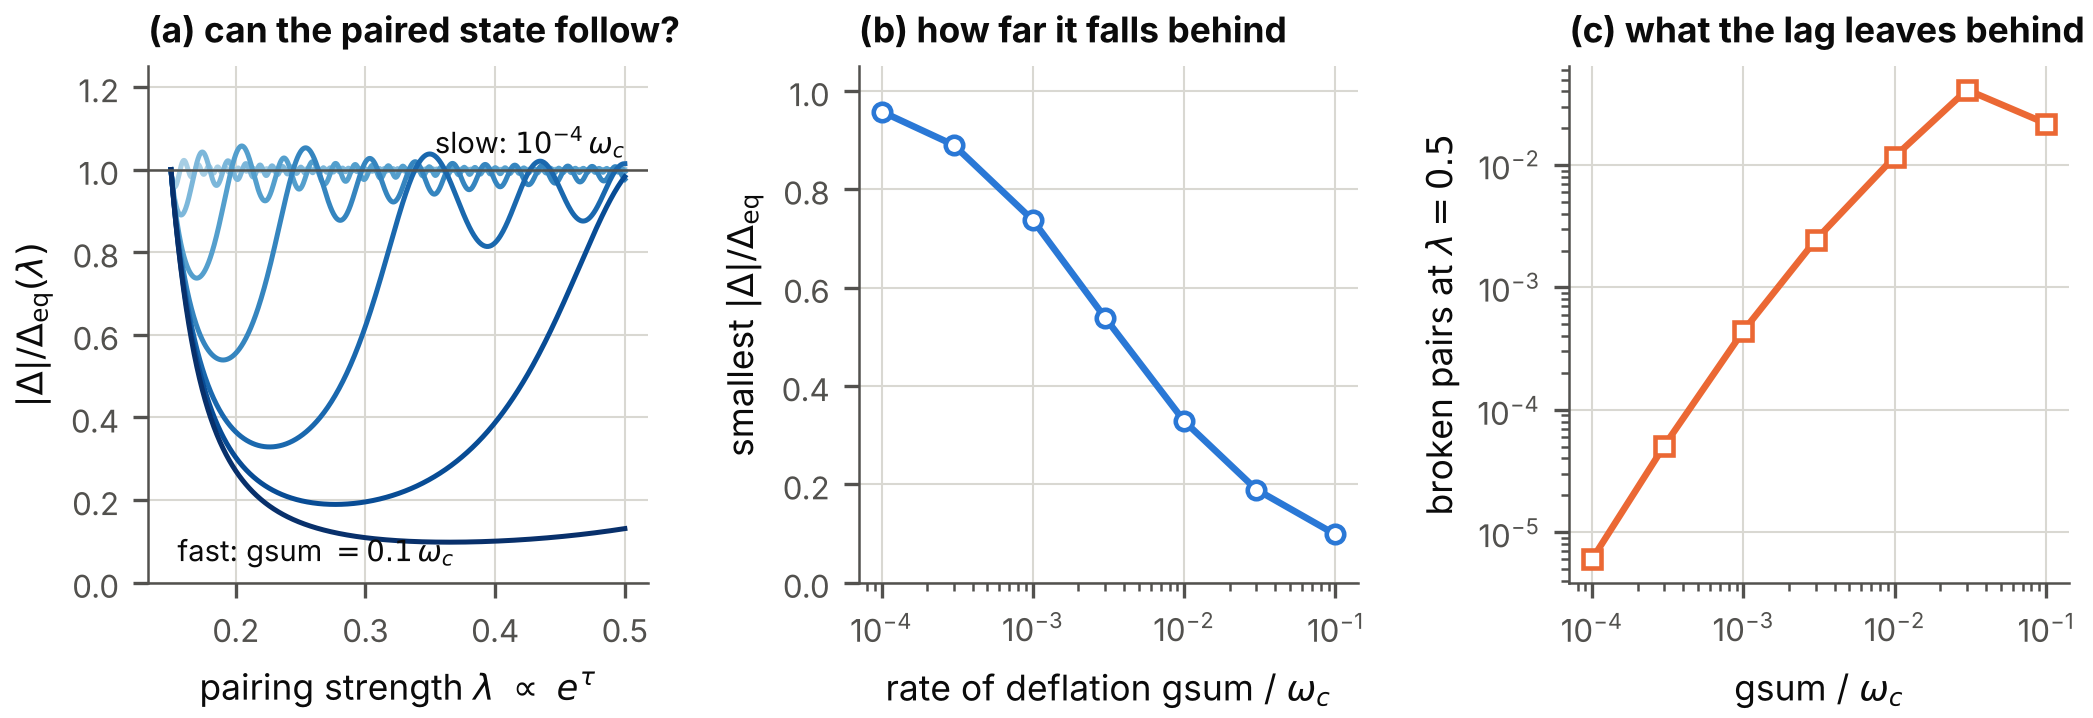
\includegraphics[width=1\textwidth,height=\textheight]{../figures/fig_quench.png}
\caption{The paired state while the coupling grows. (a) The order
parameter divided by the equilibrium gap of the moment, against the
pairing strength, for seven rates of deflation. (b) The smallest value
of that ratio against the rate. (c) The density of broken pairs at the
end of the run against the rate. Data:
\texttt{data/quench\_history.csv}, \texttt{data/quench\_summary.csv};
program: \texttt{deflation\ quench}.}
\end{figure}

\begin{center}\rule{0.5\linewidth}{0.5pt}\end{center}

\hypertarget{what-has-been-established-and-what-has-not}{%
\section{8. What has been established, and what has
not}\label{what-has-been-established-and-what-has-not}}

\textbf{Established.}

\begin{enumerate}
\def\labelenumi{\arabic{enumi}.}
\tightlist
\item
  For fields that do not depend on the extra coordinates, the model of
  the main project on a deflating spacetime is the same model with the
  couplings (1.2) of the moment, exactly (Sec. 1). The masses are
  constant; the coupling \(g_{VS}\) grows as \(e^{\tau_d/2}\);
  \(\alpha_{VS}\), \(G_{VS}\), \(D_{VS}\) and \(C\) grow as
  \(e^{\tau_d}\).
\item
  The modes of the Vorton-Scalar: growth with the weight only, a static
  potential of unchanged range and of the strength of the moment,
  thermal creation on 7+1 and extinction on 4+4 for modes that depend on
  a deflating coordinate (Sec. 2).
\item
  The exchange amplitudes of all 90 pair channels are those of the main
  project times the square of the coupling of the moment; the most
  attractive channel is unchanged (Sec. 3.1).
\item
  The gap grows according to \(d\ln(\mathrm{gap})/d\tau_d=1/\lambda\) in
  weak coupling; the critical temperature follows it (Sec. 3.2).
\item
  Two fermions become bound at a definite time, at a scattering
  resonance, with a binding energy that starts quadratically; the order
  of the other events depends on \(m_s/m\) alone (Sec. 4).
\item
  The potential of the order parameter prefers no direction among the
  four frame axes; the ground states are the unitary states (Sec. 5).
\item
  A vortex line of unit winding carries four fermion zero modes, two for
  each direction along the line, on both spacetimes and at every moment;
  its energy per length falls as \(e^{-\tau_d}\) (Sec. 6).
\item
  The paired state follows the deflation if and only if
  \(\Xi_d=\mathrm{gsum}/(\lambda\Delta_{\rm eq})\) is below about 0.2 to
  0.5; before that it lags and accumulates broken pairs (Sec. 7).
\end{enumerate}

\textbf{Not established.}

\begin{enumerate}
\def\labelenumi{\arabic{enumi}.}
\tightlist
\item
  \emph{The end of the history.} The couplings grow without bound. The
  four-dimensional description with one-boson exchange holds only while
  \(\alpha_{VS}\) is not large, and the eight-dimensional theory itself
  is an effective theory (its couplings have negative dimensions of
  mass, S1, Sec. 1.3) that must fail when the proper size of the
  deflating coordinates reaches its scale of validity. What happens then
  is outside the model.
\item
  \emph{The source and the energy.} The deflation is prescribed (DMD,
  Part 6). The energy of matter is not conserved while the couplings
  change; where it goes --- into the agent that drives the deflation ---
  is not described.
\item
  \emph{Dissipation.} The model of Sec. 7 has none. With dissipation the
  broken pairs would relax; without a calculation of the relaxation time
  nothing can be said about how long they survive.
\item
  \emph{The dynamics at the binding.} Sec. 4.1 shows that the pair
  cannot follow the deflation adiabatically at the moment of binding.
  The corresponding time-dependent two-body problem --- how much of the
  population ends in the bound state --- has not been solved.
\item
  \emph{Vortons.} The ingredients are established (Sec. 6); the
  equilibrium of a loop on the deflating spacetime, and its stability,
  are not.
\item
  \emph{Quantities beyond the mean field.} As in the main project, the
  gap equation is the two-loop truncation of the effective action
  (supplement RS4), valid in weak coupling. The late part of every
  history, where the gap is comparable with the Fermi energy, is outside
  its range of validity; the numbers there indicate the trend only.
\item
  \emph{The choice of the fields.} That the fields do not depend on
  \(x0\) is assumed, as in the main project. That they do not depend on
  \(x5,x6,x7\) is derived on 4+4 (up to the condition of admissibility
  discussed in DMD, Part 6) and assumed on 7+1, where modes that depend
  on those coordinates are populated thermally at the temperature
  \(T_{\rm defl}\), which is negligible for any allowed rate (RS3).
\end{enumerate}

\begin{center}\rule{0.5\linewidth}{0.5pt}\end{center}

\hypertarget{appendix-a.-complete-output-of-the-programs}{%
\section{Appendix A. Complete output of the
programs}\label{appendix-a.-complete-output-of-the-programs}}

\hypertarget{a.1-deflation-history}{%
\subsection{\texorpdfstring{A.1
\texttt{deflation\ history}}{A.1 deflation history}}\label{a.1-deflation-history}}

\begin{Shaded}
\begin{Highlighting}[]
\NormalTok{PROJECT spacetimes, Revision\_Deflation: checks of the history of the model along the deflation clock (couplings that grow as exp(gsum x4))}
\NormalTok{generated by: deflation (Rust crate spacetimes{-}deflation, version 0.1.0; PROJECT spacetimes, Revision\_Deflation); command: deflation history}
\NormalTok{8 of 8 checks passed}

\NormalTok{[PASS] def{-}H1  (numerical) thresholds of the model, computed again: a pair of fermions is bound if D\_VS \textgreater{} 1.67981; matter is self{-}bound if C \textgreater{} 3.7011 (3 pi\^{}2/8 = 3.7011) or, with the negative{-}energy states, C \textgreater{} 5.9218 (3 pi\^{}2/5 = 5.9218). On a deflating spacetime D\_VS and C grow as exp(gsum x4), so each threshold is passed at a definite x4}
\NormalTok{[PASS] def{-}H2  (numerical) along the clock, wherever the gap is below 0.05 E\_F the critical temperature is 0.567 times the gap (largest deviation 0.0020); the gap of the vector channel is at every moment at least as large as the gap with the radial mode alone, and that at least as large as the gap of the two{-}form channel; the gap never decreases as the deflation proceeds (four sets of m\_s/m and k\_F/m, 34 moments each)}
\NormalTok{[PASS] def{-}H3  (numerical) growth of the gap: for a weakly coupled state the gap is proportional to exp({-}1/lambda), where lambda = lambda\_S + lambda\_P is the sum of the pairing strengths of the radial mode and of the phase mode in the vector channel, and lambda grows as exp(tau\_d), which gives d ln(gap)/d tau\_d = 1/lambda; in the computed histories lambda d ln(gap)/d tau\_d lies between 1.00 and 1.03 wherever 1e{-}6 \textless{} gap/E\_F \textless{} 0.02: the gap grows much faster than the couplings, by one e{-}folding in the time 1/(gsum/lambda)}
\NormalTok{[PASS] def{-}H4  (numerical) the moment at which a pair becomes bound: just below D\_c the scattering length is large and negative ({-}134.0/m\_s at 0.99 D\_c), just above large and positive (135.9/m\_s at 1.01 D\_c); the binding energy starts as a power of the distance from the threshold with the exponents 2.01 (between 2 and 4 per cent above D\_c) and 2.01 (between 4 and 8 per cent), that is quadratically: E\_b \textasciitilde{} (exp(tau\_pair) {-} 1)\^{}2 m\_s\^{}2/m. Because E\_b vanishes at the threshold, the pair cannot follow the deflation adiabatically at first, however slow the deflation is}
\NormalTok{[PASS] def{-}H5  (numerical) matter of fixed density loses the fermion mass (the Vorton{-}Scalar loses its expectation value in the matter) when C passes a critical value that falls with the density: k\_F = 0.2 m: C = 151.892 (2.46 times pi\^{}2 m\^{}2/(4 k\_F\^{}2)); k\_F = 0.5 m: C = 12.971 (1.31 times pi\^{}2 m\^{}2/(4 k\_F\^{}2)); k\_F = 1 m: C = 2.556 (1.04 times pi\^{}2 m\^{}2/(4 k\_F\^{}2)); k\_F = 2 m: C = 0.617 (1.00 times pi\^{}2 m\^{}2/(4 k\_F\^{}2)). The estimate C = pi\^{}2 m\^{}2/(4 k\_F\^{}2) of the main project is reached at high density, where the transition happens at weak coupling; at low density the critical C is larger. On a deflating spacetime every piece of matter becomes abnormal at a definite x4, the denser the earlier}
\NormalTok{[PASS] def{-}H6  (numerical) the field beyond which the one{-}loop potential of the Vorton{-}Scalar lies below its vacuum value decreases monotonically as C grows: 24.7 v\_VS at C = 1, 1.77 v\_VS at C = 10. As the deflation proceeds the barrier that protects the vacuum moves in towards the vacuum value}
\NormalTok{[PASS] def{-}H7  (numerical) the temperature T\_half at which the fermions lose half of their mass, in units of the (constant) fermion mass, falls monotonically as g\_VS grows, for m\_s/m = 0.3, 1 and 3 (26 of the 30 moments examined; it is of the order of the four{-}dimensional vacuum value m/g\_VS, which falls as exp({-}gsum x4/2)): matter of a fixed temperature melts at a definite x4. No melting temperature can be given for m\_s/m = 0.3 from g\_VS = 1.69 (C = 32) on; there the Hartree potential ceases to exist at 1.05 v\_VS before the expectation value has fallen, because the one{-}loop potential turns over too close to the vacuum value}
\NormalTok{[PASS] def{-}H8  (numerical) order of events: the pair of fermions becomes bound before the one{-}loop potential of the Vorton{-}Scalar has fallen below its vacuum value at a field of 3 v\_VS only for the mass ratios m\_s/m = 10, 30 of the six ratios 0.1, 0.3, 1, 3, 10, 30 examined (the condition is 4 pi D\_c m/m\_s \textless{} 4.27, i.e. m\_s/m \textgreater{} 4.9): for a light radial mode the deflation destabilizes the vacuum first}
\NormalTok{[PASS] ALL  (numerical) every check above passed}
\end{Highlighting}
\end{Shaded}

\hypertarget{a.2-deflation-channels}{%
\subsection{\texorpdfstring{A.2
\texttt{deflation\ channels}}{A.2 deflation channels}}\label{a.2-deflation-channels}}

\begin{Shaded}
\begin{Highlighting}[]
\NormalTok{PROJECT spacetimes, Revision\_Deflation: checks of the exchange of the Vorton{-}Scalar on the deflating spacetimes (def{-}K..: amplitudes in the pair channels; def{-}B..: the exchanged field)}
\NormalTok{generated by: deflation (Rust crate spacetimes{-}deflation, version 0.1.0; PROJECT spacetimes, Revision\_Deflation); command: deflation channels}
\NormalTok{7 of 7 checks passed}

\NormalTok{[PASS] def{-}K1  (numerical) the exchange amplitudes of the Vorton{-}Scalar in 90 pair channels (both spacetimes, three momenta, 13 angles: 1170 rows) computed again with the frame matrices agree with every number of the file data/pair\_channel\_kernel.csv of the main project to the digits printed there (1170 rows compared). For fields that do not depend on x5, x6, x7 the amplitude of a channel on the deflating spacetime is the flat amplitude times the square of the coupling of the moment}
\NormalTok{[PASS] def{-}K2  (numerical) the amplitudes of the hidden{-}axis channel reproduce the closed forms of the main project (largest deviation 1.1e{-}15)}
\NormalTok{[PASS] def{-}K3  (numerical) the quartic invariant of the gap matrix of the four vector pairs, Tr[(M\_gap M\_gap\^{}dagger)\^{}2]/8 = 2 (sum |Delta\^{}a|\^{}2)\^{}2 {-} |eta\_ab Delta\^{}a Delta\^{}b|\^{}2 with the frame metric of x0, x5, x6, x7, holds on both deflating spacetimes (largest deviation 2.1e{-}14); in coordinate components Delta\_t = b\_t(x4) Delta\^{}t the same form reads with the metric g\_tt of the moment}
\NormalTok{[PASS] def{-}B1  (numerical) the field that a static source builds up from zero approaches exp(gsum x4)/(k\^{}2 + m\_bos\^{}2): after tau\_d = gsum x4 = 20 the relative difference is 1.9e{-}5 4.3e{-}6 2.4e{-}5 3.5e{-}5 for (k\^{}2 + m\_bos\^{}2, gsum) = (1, 0.2), (0.25, 0.2), (1, 1), (4, 0.5) (transient proportional to exp({-}tau\_d/2)). The potential between two fermions at rest is therefore the Yukawa potential of the unshifted mass m\_s with the strength alpha\_VS of the moment}
\NormalTok{[PASS] def{-}B2  (exact) a mode of the Vorton{-}Scalar that does not depend on x5, x6, x7 goes as exp(exponent x4) with exponent = gsum/2 +{-} sqrt(gsum\^{}2/4 {-} k\^{}2 {-} m\_bos\^{}2): it oscillates if and only if k\^{}2 + m\_bos\^{}2 \textgreater{} gsum\^{}2/4, and its amplitude then grows as exp(gsum x4/2) (the weighted field has constant amplitude: the number of quanta is conserved). The phase mode (m\_bos = 0) does not oscillate for k \textless{} gsum/2; the radial mode oscillates at every k if m\_s \textgreater{} gsum/2 (table data/scalar\_zero\_modes.csv)}
\NormalTok{[PASS] def{-}B3  (numerical) 7+1: a mode of the Vorton{-}Scalar that depends on one deflating coordinate and starts empty ends with 1/(exp(2 pi varpi\_b/rate\_t) {-} 1) quanta, a Bose{-}Einstein law with the temperature rate\_t/(2 pi): 36 cases (varpi\_b/rate\_t = 0.25 to 3, each of the three coordinates), largest relative deviation 1.9e{-}5; the Bogoliubov coefficients satisfy |alpha|\^{}2 {-} |beta|\^{}2 = 1 to 1.3e{-}13}
\NormalTok{[PASS] def{-}B4  (numerical) 4+4: a mode of the Vorton{-}Scalar that depends on a deflating time has one bounded solution; at early x4 it is a standing wave (the two travelling waves have equal amplitudes) and its profile is the modified Bessel function K of the imaginary order i varpi\_b/rate\_t (ratio to the exact form constant to 1e{-}4 away from the zeros): varpi\_b/rate\_t = 0.5: |c\_{-}/c\_+| {-} 1 = 0.0e0, 23 of 23 samples; varpi\_b/rate\_t = 1.5: |c\_{-}/c\_+| {-} 1 = 0.0e0, 24 of 24 samples; varpi\_b/rate\_t = 3: |c\_{-}/c\_+| {-} 1 = 0.0e0, 26 of 26 samples;}
\NormalTok{[PASS] ALL  (numerical) every check above passed}
\end{Highlighting}
\end{Shaded}

\hypertarget{a.3-deflation-quench}{%
\subsection{\texorpdfstring{A.3
\texttt{deflation\ quench}}{A.3 deflation quench}}\label{a.3-deflation-quench}}

\begin{Shaded}
\begin{Highlighting}[]
\NormalTok{PROJECT spacetimes, Revision\_Deflation: checks of the time{-}dependent dynamics of the paired state under a coupling that grows as exp(gsum x4)}
\NormalTok{generated by: deflation (Rust crate spacetimes{-}deflation, version 0.1.0; PROJECT spacetimes, Revision\_Deflation); command: deflation quench}
\NormalTok{5 of 5 checks passed}

\NormalTok{[PASS] def{-}Q1  (numerical) the equations of motion conserve |2F|\^{}2 + (1 {-} 2n)\^{}2 = 1 for every pair: largest deviation at the end of the seven runs 4.2e{-}11}
\NormalTok{[PASS] def{-}Q2  (numerical) convergence: with twice as many energies (4000) and half the time step the run with gsum = 1e{-}3 E\_sh gives the smallest ratio 0.73710 (against 0.73710) and the final density of broken pairs 4.4255e{-}4 (against 4.4255e{-}4)}
\NormalTok{[PASS] def{-}Q3  (numerical) the faster the deflation, the further the order parameter falls behind: the smallest value of |Delta|/Delta\_eq is 0.958, 0.890, 0.737, 0.539, 0.328, 0.189, 0.098 for gsum/E\_sh = 1e{-}4, 3e{-}4, 1e{-}3, 3e{-}3, 1e{-}2, 3e{-}2, 1e{-}1 (Xi\_d at the start: 0.26 to 262)}
\NormalTok{[PASS] def{-}Q4  (numerical) the order parameter catches up with the equilibrium gap of the moment (to within 10 per cent) when Xi\_d = gsum/(lambda Delta\_eq) has fallen to a value between 0.23 and 0.52 (six runs; in the fastest run, gsum = 0.1 E\_sh, it does not catch up before lambda = 0.5): the paired state follows the deflation if and only if gsum is small compared with lambda times the gap}
\NormalTok{[PASS] def{-}Q5  (numerical) the lag leaves broken pairs behind: their density at lambda = 0.5 is 6.0e{-}6, 5.1e{-}5, 4.4e{-}4, 2.4e{-}3, 1.2e{-}2, 4.1e{-}2 (units of E\_sh times the density of states) for gsum/E\_sh = 1e{-}4 to 3e{-}2, growing with the rate; for the equilibrium state it is zero}
\NormalTok{[PASS] ALL  (numerical) every check above passed}
\end{Highlighting}
\end{Shaded}

\hypertarget{a.4-deflation-symmetry}{%
\subsection{\texorpdfstring{A.4
\texttt{deflation\ symmetry}}{A.4 deflation symmetry}}\label{a.4-deflation-symmetry}}

The checks \texttt{44d-S..}, \texttt{71d-S..} are discussed in DMD, Part
5, and in the supplement RS2.

\begin{Shaded}
\begin{Highlighting}[]
\NormalTok{PROJECT spacetimes, Revision\_Deflation: checks of the symmetries on the deflating spacetimes (isometries, internal symmetry of the fields that do not depend on the extra coordinates, zero modes on a vortex line, reduction of the couplings)}
\NormalTok{generated by: deflation (Rust crate spacetimes{-}deflation, version 0.1.0; PROJECT spacetimes, Revision\_Deflation); command: deflation symmetry}
\NormalTok{18 of 18 checks passed}

\NormalTok{[PASS] 44d{-}S1  (exact) of the 28 rotations and boosts of the flat 4+4 spacetime (one for each pair of coordinates) exactly 6 remain isometries of the deflating spacetime for three different rates (the rotations of x0, x1, x2, x3), 7 if two rates are equal (in addition the rotation of the two coordinates that deflate at the same rate) and 9 if the three rates are equal (in addition the three rotations of x5, x6, x7); no transformation that involves x4 survives, and none that mixes x0 with a deflating coordinate. Together with the 7 translations, the scaling and, for equal rates, the three special vectors of metric.rs this gives 14, 15 and 20 Killing vectors (Lie derivative of the metric zero at two points, exact arithmetic)}
\NormalTok{[PASS] 44d{-}S2  (exact) the products gamma\^{}A gamma\^{}B that commute with the five matrices alpha\^{}1, alpha\^{}2, alpha\^{}3, beta, i beta chi (and so act as internal symmetries on fields that do not depend on the extra coordinates) are exactly those of the six pairs taken from x0, x5, x6, x7. Of these six, the deflating spacetime keeps as isometries 0 (three different rates), 1 (two equal rates) and 3 (three equal rates): the remaining 6, 5 and 3 are symmetries of the sector of such fields that have no counterpart among the isometries of the spacetime (hidden symmetries)}
\NormalTok{[PASS] 71d{-}S1  (exact) of the 28 rotations and boosts of the flat 7+1 spacetime (one for each pair of coordinates) exactly 6 remain isometries of the deflating spacetime for three different rates (the rotations of x0, x1, x2, x3), 7 if two rates are equal (in addition the rotation of the two coordinates that deflate at the same rate) and 9 if the three rates are equal (in addition the three rotations of x5, x6, x7); no transformation that involves x4 survives, and none that mixes x0 with a deflating coordinate. Together with the 7 translations, the scaling and, for equal rates, the three special vectors of metric.rs this gives 14, 15 and 20 Killing vectors (Lie derivative of the metric zero at two points, exact arithmetic)}
\NormalTok{[PASS] 71d{-}S2  (exact) the products gamma\^{}A gamma\^{}B that commute with the five matrices alpha\^{}1, alpha\^{}2, alpha\^{}3, beta, i beta chi (and so act as internal symmetries on fields that do not depend on the extra coordinates) are exactly those of the six pairs taken from x0, x5, x6, x7. Of these six, the deflating spacetime keeps as isometries 0 (three different rates), 1 (two equal rates) and 3 (three equal rates): the remaining 6, 5 and 3 are symmetries of the sector of such fields that have no counterpart among the isometries of the spacetime (hidden symmetries)}
\NormalTok{[PASS] def{-}S3  (numerical) the internal symmetry of the fields that do not depend on the extra coordinates, computed again for both spacetimes (24 items of data/reduced\_symmetry.csv, all as expected): the commutant of the five matrices has dimension 8 and is u(2) + u(2) = su(2)\_A + su(2)\_B + u(1)\_F + u(1)\_E; the eight one{-}particle states are (2,1) + (1,2); the four vector pair operators are the (2,2) with fermion number 2, and their invariant quadratic form is the frame metric of the axes x0, x5, x6, x7. The deflation does not change this symmetry, because the weighted field of this sector obeys the flat equations (checks 44d{-}D.., 71d{-}D.. of the command matrices)}
\NormalTok{[PASS] 44d{-}V1  (exact) alpha\^{}1, alpha\^{}2, alpha\^{}3, beta and i beta chi are Hermitian, have square one and anticommute with one another}
\NormalTok{[PASS] 44d{-}V2  (exact) i beta alpha\^{}1 and alpha\^{}2 beta chi are commuting Hermitian matrices with square one}
\NormalTok{[PASS] 44d{-}V3  (exact) each of the four joint eigenspaces of the two matrices has dimension 4: a vortex line of unit winding carries four zero modes of the sixteen{-}component field}
\NormalTok{[PASS] 44d{-}V4  (exact) Pc = i alpha\^{}1 alpha\^{}2 alpha\^{}3 chi equals the product of the five matrices, commutes with each of them, is Hermitian and traceless and has square one: it is, up to sign, the generator P of U(1)\_E}
\NormalTok{[PASS] 44d{-}V5  (exact) winding +1: every w\_z with (i beta alpha\^{}1) w\_z = {-}w\_z, (alpha\^{}2 beta chi) w\_z = {-}w\_z solves the zero{-}energy equations (i alpha\^{}1 + beta) w\_z = 0, (i alpha\^{}2 + i beta chi) w\_z = 0; on these four spinors alpha\^{}3 = Pc, and its trace vanishes: two zero modes have alpha\^{}3 = +1 (energy +k\_3) and two alpha\^{}3 = {-}1 (energy {-}k\_3)}
\NormalTok{[PASS] 44d{-}V6  (exact) winding {-}1: the spinors w\_z with (i beta alpha\^{}1) w\_z = {-}w\_z, (alpha\^{}2 beta chi) w\_z = +w\_z solve (i alpha\^{}1 + beta) w\_z = 0, (i alpha\^{}2 {-} i beta chi) w\_z = 0, and on them alpha\^{}3 = {-}Pc: the directions of motion are exchanged}
\NormalTok{[PASS] 71d{-}V1  (exact) alpha\^{}1, alpha\^{}2, alpha\^{}3, beta and i beta chi are Hermitian, have square one and anticommute with one another}
\NormalTok{[PASS] 71d{-}V2  (exact) i beta alpha\^{}1 and alpha\^{}2 beta chi are commuting Hermitian matrices with square one}
\NormalTok{[PASS] 71d{-}V3  (exact) each of the four joint eigenspaces of the two matrices has dimension 4: a vortex line of unit winding carries four zero modes of the sixteen{-}component field}
\NormalTok{[PASS] 71d{-}V4  (exact) Pc = i alpha\^{}1 alpha\^{}2 alpha\^{}3 chi equals the product of the five matrices, commutes with each of them, is Hermitian and traceless and has square one: it is, up to sign, the generator P of U(1)\_E}
\NormalTok{[PASS] 71d{-}V5  (exact) winding +1: every w\_z with (i beta alpha\^{}1) w\_z = {-}w\_z, (alpha\^{}2 beta chi) w\_z = {-}w\_z solves the zero{-}energy equations (i alpha\^{}1 + beta) w\_z = 0, (i alpha\^{}2 + i beta chi) w\_z = 0; on these four spinors alpha\^{}3 = Pc, and its trace vanishes: two zero modes have alpha\^{}3 = +1 (energy +k\_3) and two alpha\^{}3 = {-}1 (energy {-}k\_3)}
\NormalTok{[PASS] 71d{-}V6  (exact) winding {-}1: the spinors w\_z with (i beta alpha\^{}1) w\_z = {-}w\_z, (alpha\^{}2 beta chi) w\_z = +w\_z solve (i alpha\^{}1 + beta) w\_z = 0, (i alpha\^{}2 {-} i beta chi) w\_z = 0, and on them alpha\^{}3 = {-}Pc: the directions of motion are exchanged}
\NormalTok{[PASS] def{-}S4  (exact) reduction to fields that do not depend on x5, x6, x7: sqrt|g| times the Yukawa term and the potential of the Vorton{-}Scalar, written with the weighted fields psihat = sqrt(Vd) psi and Phihat = sqrt(Vd) Phi\_VS, are the same expressions with the couplings y\_VS/sqrt(Vd), lambda\_VS/Vd and the vacuum value v\_VS sqrt(Vd); the products y\_VS v\_VS and lambda\_VS v\_VS\^{}2, hence the fermion mass and the mass of the radial mode, do not change (rational sample values, exact). The exponents of data/coupling\_exponents.csv follow, with Vd proportional to exp({-}gsum x4)}
\NormalTok{[PASS] ALL  (exact) every check above passed}
\end{Highlighting}
\end{Shaded}

\hypertarget{appendix-b.-files}{%
\section{Appendix B. Files}\label{appendix-b.-files}}

\begin{longtable}[]{@{}
  >{\raggedright\arraybackslash}p{(\columnwidth - 4\tabcolsep) * \real{0.1905}}
  >{\raggedright\arraybackslash}p{(\columnwidth - 4\tabcolsep) * \real{0.6190}}
  >{\raggedright\arraybackslash}p{(\columnwidth - 4\tabcolsep) * \real{0.1905}}@{}}
\toprule\noalign{}
\begin{minipage}[b]{\linewidth}\raggedright
file
\end{minipage} & \begin{minipage}[b]{\linewidth}\raggedright
content
\end{minipage} & \begin{minipage}[b]{\linewidth}\raggedright
written by
\end{minipage} \\
\midrule\noalign{}
\endhead
\bottomrule\noalign{}
\endlastfoot
\texttt{code/deflation-rs/src/history.rs} & couplings along the clock;
gap, pair, matter, vacuum and temperature at each moment & --- \\
\texttt{code/deflation-rs/src/scalar.rs} & modes of the scalar:
exponents, static source, creation, bounded solutions & --- \\
\texttt{code/deflation-rs/src/quench.rs} & time-dependent mean-field
dynamics of the shell model & --- \\
\texttt{code/deflation-rs/src/symmetry\_defl.rs} & algebra of the vortex
zero modes; reduction of the couplings & --- \\
\texttt{code/deflation-rs/src/cmd\_channels.rs} & exchange amplitudes on
the deflating spacetimes; quartic invariant & --- \\
\texttt{data/coupling\_exponents.csv} & the exponents of Sec. 1.3 &
\texttt{deflation\ symmetry} \\
\texttt{data/events.csv} & the order of events of Sec. 4.2 &
\texttt{deflation\ history} \\
\texttt{data/gap\_history.csv} & the gap along the clock, four sets &
\texttt{deflation\ history} \\
\texttt{data/dimer\_history.csv} & scattering length and binding energy
along the clock & \texttt{deflation\ history} \\
\texttt{data/pair\_channel\_kernel.csv},
\texttt{data/gl\_quartic\_check.csv} & exchange amplitudes; the identity
(5.1) & \texttt{deflation\ channels} \\
\texttt{data/scalar\_zero\_modes.csv}, \texttt{data/static\_source.csv}
& Sec. 2.1 and 2.2 & \texttt{deflation\ channels} \\
\texttt{data/boson\_creation.csv}, \texttt{data/boson\_bounded.csv} &
Sec. 2.3 & \texttt{deflation\ channels} \\
\texttt{data/quench\_history.csv}, \texttt{data/quench\_summary.csv} &
Sec. 7 & \texttt{deflation\ quench} \\
\texttt{data/order\_parameter\_states.csv} & Sec. 5.2 &
\texttt{deflation\ paired} \\
\texttt{data/history\_checks.txt}, \texttt{channel\_checks.txt},
\texttt{quench\_checks.txt}, \texttt{symmetry\_checks.txt} (and
\texttt{.csv}) & Appendix A & the four commands \\
\texttt{figures/fig\_clock}, \texttt{fig\_scalar},
\texttt{fig\_kernels}, \texttt{fig\_gap\_history},
\texttt{fig\_binding}, \texttt{fig\_quench} (\texttt{.pdf},
\texttt{.png}) & the six figures & \texttt{make\_figures.py} \\
\end{longtable}

\end{document}
